\documentclass[12pt,(landscape,a4paper),(portrait,a4paper)]{article}
\usepackage{lmodern}
\usepackage{amssymb,amsmath}
\usepackage{ifxetex,ifluatex}
\usepackage{fixltx2e} % provides \textsubscript
\ifnum 0\ifxetex 1\fi\ifluatex 1\fi=0 % if pdftex
  \usepackage[T1]{fontenc}
  \usepackage[utf8]{inputenc}
\else % if luatex or xelatex
  \ifxetex
    \usepackage{mathspec}
  \else
    \usepackage{fontspec}
  \fi
  \defaultfontfeatures{Ligatures=TeX,Scale=MatchLowercase}
\fi
% use upquote if available, for straight quotes in verbatim environments
\IfFileExists{upquote.sty}{\usepackage{upquote}}{}
% use microtype if available
\IfFileExists{microtype.sty}{%
\usepackage{microtype}
\UseMicrotypeSet[protrusion]{basicmath} % disable protrusion for tt fonts
}{}
\usepackage[margin=1in]{geometry}
\usepackage{hyperref}
\hypersetup{unicode=true,
            pdftitle={计量经济学Eviews实验指导书},
            pdfauthor={胡华平},
            pdfborder={0 0 0},
            breaklinks=true}
\urlstyle{same}  % don't use monospace font for urls
\usepackage{longtable,booktabs}
\usepackage{graphicx,grffile}
\makeatletter
\def\maxwidth{\ifdim\Gin@nat@width>\linewidth\linewidth\else\Gin@nat@width\fi}
\def\maxheight{\ifdim\Gin@nat@height>\textheight\textheight\else\Gin@nat@height\fi}
\makeatother
% Scale images if necessary, so that they will not overflow the page
% margins by default, and it is still possible to overwrite the defaults
% using explicit options in \includegraphics[width, height, ...]{}
\setkeys{Gin}{width=\maxwidth,height=\maxheight,keepaspectratio}
\IfFileExists{parskip.sty}{%
\usepackage{parskip}
}{% else
\setlength{\parindent}{0pt}
\setlength{\parskip}{6pt plus 2pt minus 1pt}
}
\setlength{\emergencystretch}{3em}  % prevent overfull lines
\providecommand{\tightlist}{%
  \setlength{\itemsep}{0pt}\setlength{\parskip}{0pt}}
\setcounter{secnumdepth}{0}
% Redefines (sub)paragraphs to behave more like sections
\ifx\paragraph\undefined\else
\let\oldparagraph\paragraph
\renewcommand{\paragraph}[1]{\oldparagraph{#1}\mbox{}}
\fi
\ifx\subparagraph\undefined\else
\let\oldsubparagraph\subparagraph
\renewcommand{\subparagraph}[1]{\oldsubparagraph{#1}\mbox{}}
\fi

%%% Use protect on footnotes to avoid problems with footnotes in titles
\let\rmarkdownfootnote\footnote%
\def\footnote{\protect\rmarkdownfootnote}

%%% Change title format to be more compact
\usepackage{titling}

% Create subtitle command for use in maketitle
\newcommand{\subtitle}[1]{
  \posttitle{
    \begin{center}\large#1\end{center}
    }
}

\setlength{\droptitle}{-2em}

  \title{计量经济学Eviews实验指导书}
    \pretitle{\vspace{\droptitle}\centering\huge}
  \posttitle{\par}
  \subtitle{Lab 8 虚拟变量回归模型}
  \author{胡华平}
    \preauthor{\centering\large\emph}
  \postauthor{\par}
      \predate{\centering\large\emph}
  \postdate{\par}
    \date{2018/5/4}

\usepackage{xeCJK}
\setCJKmainfont{楷体}  % 字体可以更换
\setmainfont{Georgia} % 設定英文字型
\setromanfont{Georgia} % 字型
\setmonofont{Courier New}

%设置版式 垂直或水平
% You know, for landscape
\usepackage{lscape}
\usepackage{pdfpages}


% Make new page before each section
\let\stdsection\section
\renewcommand\section{\newpage\stdsection}

% pandoc does not parse latex env - https://groups.google.com/forum/?fromgroups=#!topic/pandoc-discuss/oZETB5Ii1Cw
\newcommand{\blandscape}{\begin{landscape}}
\newcommand{\elandscape}{\end{landscape}}

\usepackage{amsthm}
\newtheorem{theorem}{Theorem}
\newtheorem{lemma}{Lemma}
\newtheorem{corollary}{Corollary}
\newtheorem{proposition}{Proposition}
\newtheorem{conjecture}{Conjecture}
\theoremstyle{definition}
\newtheorem{definition}{Definition}
\theoremstyle{definition}
\newtheorem{example}{Example}
\theoremstyle{definition}
\newtheorem{exercise}{Exercise}
\theoremstyle{remark}
\newtheorem*{remark}{Remark}
\newtheorem*{solution}{Solution}
\let\BeginKnitrBlock\begin \let\EndKnitrBlock\end
\begin{document}
\maketitle

\renewcommand{\figurename}{图}
\renewcommand{\contentsname}{目录}
\renewcommand{\tablename}{表}


%% maxwidth is the original width if it's less than linewidth
%% otherwise use linewidth (to make sure the graphics do not exceed the margin)
\makeatletter
\def\maxwidth{ %
  \ifdim\Gin@nat@width>\linewidth
    \linewidth
  \else
    \Gin@nat@width
  \fi
}
\makeatother

{
\setcounter{tocdepth}{5}
\tableofcontents
}
\newpage

\hypertarget{dummy-variable}{%
\section{虚拟变量回归模型}\label{dummy-variable}}

\subsection{实验目的及要求}

\begin{itemize}
\tightlist
\item
  \textbf{目的}:掌握虚拟变量模型的设置和分析方法。
\item
  \textbf{要求}:熟悉虚拟变量的设置方法;理解定性变量和定量变量模型的内涵;熟练加法模型和乘法模型的运用原理。
\end{itemize}

\subsection{实验原理}

计量经济学建模分析中,我们常常需要把一些\textbf{定性变量(Qualitative
variables)}(如性别、地区、党派等)作为自变量放入回归模型中。从\textbf{变量层次(Variable
Scale)}来看,这些变量没有具体的取值,只有特定属性类别。例如,性别变量的具体取值往往为男或女。显然,诸如此类的变量如果直接放到线性回归模型中,将会产生一系列的参数估计、模型解释等问题。

\BeginKnitrBlock{definition}[定量变量]
\protect\hypertarget{def:var-quanty}{}{\label{def:var-quanty}
\iffalse (定量变量) \fi{} }定量变量(Quantitative
variable)一般也称为连续变量,是由测量或计数、统计所得到的量,可以通过数值表达,并具有直接的数值含义。
\EndKnitrBlock{definition}

\BeginKnitrBlock{definition}[定性变量]
\protect\hypertarget{def:var-quality}{}{\label{def:var-quality}
\iffalse (定性变量) \fi{} }定性变量(Qualitative
variable)一般也称为分类变量,主要用于区分事物性质差异,往往用语义类别表达,没有直接的数值含义。
\EndKnitrBlock{definition}

\BeginKnitrBlock{definition}[变量尺度]
\protect\hypertarget{def:var-scale}{}{\label{def:var-scale}
\iffalse (变量尺度) \fi{} }变量尺度(Variable
scale)刻画的是变量的数值含义或数值关系。它将意味着在数值含义和关系上,变量是有层次级别的差异性。根据变量层级不同,具体可以分为由低到高的4个层级:
\textbf{名义尺度(nominal
scale)变量}:这类变量只用于属性分类,不具备任何数值含义或数值关系,也即不能加、减、乘、除,也不能比较大小。
\textbf{序数尺度(order
scale)变量}:这类变量具备很少的数值含义或数值关系,它可以比较大小,但不能进行加、减、乘、除。
\textbf{区间尺度(interval
scale)变量}:这类变量具备一定的数值含义或数值关系,它可以比较大小,也可以进行加、减,但不能进行乘、除。
\textbf{比率尺度(ratio
scale)变量}:这类变量具备最多的数值含义或数值关系,它可以比较大小,也可以进行加、减、乘、除。
\EndKnitrBlock{definition}

\subsubsection{如何把定性变量转换为虚拟变量?}

一个定性变量的不同数据取值,称为该定性变量的属性。定性变量的任一属性,都可以设置为一个\textbf{虚拟变量}。实际上,我们可以用一套\textbf{虚拟变量体系}来完全表达一个定性变量。然后按照一定的规则构建\textbf{虚拟变量回归模型},从而避免参数估计、模型解释等问题的出现。

\BeginKnitrBlock{definition}[虚拟变量]
\protect\hypertarget{def:var-dummy}{}{\label{def:var-dummy}
\iffalse (虚拟变量) \fi{}
}对于某定性变量的任一特定属性,可以构造出一个虚拟变量(记为D),使得该虚拟变量能够表达这一属性。同时,给该虚拟变量D赋值为1,记为具备这一属性;给该虚拟变量赋值为0,记为不具备该属性。正式地,假设定性变量\(X\)具有\(m\)个属性\(a_1,a_2,\cdots,a_m\),对于任意属性\(k,(k\in{1,2,\cdots,m})\),可以定义如下的虚拟变量\(D_k\):

\begin{equation}
D_k=
\begin{cases}
1, & \text{if } a_k\\
0, & \text{if not }  a_k
\end{cases}
\end{equation}
\EndKnitrBlock{definition}

\BeginKnitrBlock{definition}[虚拟变量体系]
\protect\hypertarget{def:model-dummy}{}{\label{def:model-dummy}
\iffalse (虚拟变量体系) \fi{}
}完整表达某个定性变量全部信息的一组虚拟变量。正式地,假设定性变量\(X\)具有\(m\)个属性\(a_1,a_2,\cdots,a_m\),可以用如下一组虚拟变量\(D_1,\cdots,D_k,\cdots,D_m\)完全表达该定性变量:
\begin{align}
X\{a_1,a_2,\cdots,a_m\} \Rightarrow  
  \begin{cases}
    D_1  =
    \begin{cases}
    1, & \text{if } a_1\\
    0, & \text{if not }  a_1
    \end{cases} \\
     \vdots \\
    D_k = 
    \begin{cases}
    1, & \text{if } a_k\\
    0, & \text{if not }  a_k
    \end{cases} \\
    \vdots\\
    D_m  =
    \begin{cases}
    1, & \text{if } a_m\\
    0, & \text{if not }  a_m
    \end{cases}
  \end{cases}
\end{align}
\EndKnitrBlock{definition}

例如,定性变量肤色(\(X\))具有3个属性(\(m=3\)),具体为\(X\{a_1=yellow,a_2=white,a_3=black\}\),则可以构造出如下的虚拟变量体系\footnote{一个定性变量如果有m个属性,那么可以用m个虚拟变量\textbf{完全表达}该定性变量,也可以用\((m-1)\)个虚拟变量\textbf{充分表达}该定性变量。}:

\begin{align}
X\{a_1=\text{yellow},a_2=\text{white},a_3=\text{black}\} \\
\Longrightarrow  
  \begin{cases}
    D_1  =
    \begin{cases}
    1, & \text{yellow}\\
    0, & \text{not yellow}
    \end{cases} \\
    D_2 = 
    \begin{cases}
    1, & \text{white}\\
    0, & \text{not white}
    \end{cases} \\
    D_3  =
    \begin{cases}
    1, & \text{black}\\
    0, & \text{not black}
    \end{cases}
  \end{cases}
\end{align}

\subsubsection{如何理解虚拟变量回归模型?}

一个线性回归模型,只要回归元中包含了虚拟变量,这种模型就被称为\textbf{虚拟变量回归模型},也可以称为\textbf{方差分析模型}
(Analysis of variance, ANOVA)\footnote{\textbf{方差分析模型}(Analysis
  of variance,
  ANOVA)常用来分析定量化的因变量\(Y\)与定性回归元或虚拟变量之间的统计显著性关系。一般是通过比较不同类别或不同组的均值差,例如采用t检验可以判断两组均值是否有显著的差异}。

根据回归元包含定量变量和虚拟变量的数量关系,可以将虚拟变量回归模型分为:

\begin{itemize}
\tightlist
\item
  只含有虚拟变量的回归模型:全部解释变量都是由虚拟变量构成
\item
  同时含有虚拟变量和定量变量的回归模型:解释变量同时含有虚拟变量和定量变量
\end{itemize}

根据虚拟变量引入模型方式的不同,可以划分为:

\begin{itemize}
\tightlist
\item
  加法模型:虚拟变量以独立项的形式出现在方程中
\item
  乘法模型:虚拟变量以交叉项的形式出现在方程中
\item
  混合模型:虚拟变量以独立项和/或交叉项的形式出现在方程中\footnote{有时候模型设置中,某个虚拟变量体系(用来表达某个定性变量)的独立项可以完全不出现在方程中(也即没有它们的加法形式),而却可以出现它们与其他变量的交叉项(也即可以出现它们与其他变量的乘法形式)。}

  \begin{itemize}
  \tightlist
  \item
    完全混合模型
  \item
    部分混合模型
  \end{itemize}
\end{itemize}

根据虚拟变量模型是否参照\textbf{基础组},可以划分为\footnote{如果理论要求与\textbf{基础组}对比,则理论模型必须设置为有截距回归模型;否则,理论模型需要设置无截距回归模型。}:

\begin{itemize}
\tightlist
\item
  有截距模型:此时模型解释中将有明确的\textbf{基础组},其他组可以直接与之参照对比。
\item
  无截距模型:此时模型解释中将没有明确的\textbf{基础组},各组间将不直接参照对比。
\end{itemize}

根据模型中的因变量\(Y\)是否取对数,可以划分为\footnote{半对数或对数模型将蕴含着弹性和斜率的经济学含义,在解释虚拟变量回归模型中往往很有现实意义。}:

\begin{itemize}
\tightlist
\item
  经典线性模型:因变量为\(Y\)
\item
  半对数模型:因变量为\(ln(Y)\)
\end{itemize}

根据虚拟变量模型应用情景的不同,可以划分为:

\begin{itemize}
\tightlist
\item
  截面数据虚拟变量回归模型:此时虚拟变量用于表达回归元为定性变量的情形
\item
  时间序列季节虚拟变量回归模型:此时虚拟变量用于表达季节周期(具体请参看节\ref{seasonal})
\item
  分段线性虚拟变量回归模型:此时虚拟变量用于表达\textbf{阀值}分段(具体请参看节\ref{piecewise})
\end{itemize}

对于具体的实证分析案例,我们往往需要根据变量的属性和特征,构建不同类型的虚拟变量回归模型,比较不同模型的回归分析结果,甄选并得到其中相对理想的模型。显然,不同类型的虚拟变量模型设置,具有不同的经济学含义。甚至回归方程系数解读的直观性,模型构建意图表达的直接性等,也存在较大差异,都需要对各种备选的、可行的模型进行反复测试和甄选。

例如,仅是考虑\textbf{基础组}的有截距模型,可能用到的各类备选组合模型至少包括(具体回归方程设置见节\ref{group1}和节\ref{group2}):

\begin{itemize}
\tightlist
\item
  只含有虚拟变量的、加法形式的\textbf{经典回归模型}
\item
  只含有虚拟变量的、加法形式的\textbf{半对数回归模型}
\item
  只含有虚拟变量的、乘法形式的\textbf{经典回归模型}
\item
  只含有虚拟变量的、乘法形式的\textbf{半对数回归模型}
\item
  \(\cdots\)
\item
  同时含有虚拟变量和定量变量的、加法形式的\textbf{经典回归模型}
\item
  同时含有虚拟变量和定量变量的、加法形式的\textbf{半对数回归模型}
\item
  同时含有虚拟变量和定量变量的、乘法形式的\textbf{经典回归模型}
\item
  同时含有虚拟变量和定量变量的、乘法形式的\textbf{半对数回归模型}
\item
  \(\cdots\)
\end{itemize}

\subsection{实验内容}

\begin{enumerate}
\def\labelenumi{\arabic{enumi}.}
\item
  采用最小二乘法建立主回归模型
\item
  自相关问题模型的侦察方法

  \begin{enumerate}
  \def\labelenumii{\alph{enumii}.}
  \tightlist
  \item
    残差序列观察法(描点图法):绘制\(e_t\)序列的描点图(dot plot)\\
  \item
    残差序列观察法(描点图法):确定滞后阶数并分别绘制\(e_t\)序列与\({e_{t-1},e_{t-2},\cdots}\)序列的散点图(scatter
    plot)\\
  \item
    辅助回归法:构建残差\(e_t\)序列对\({e_{t-1},e_{t-2},\cdots}\)序列的辅助回归方程\\
  \item
    自相关和偏相关分析法:Eviews菜单操作对残差\(e_t\)序列进行自相关和偏相关分析(\textbf{注意滞后阶数的选择})
  \item
    Durbin-Watson检验法:分析Eviews报告中的D-W统计量\\
  \item
    拉格朗日检验法(LM-test):Eviews菜单操作进行布罗施-戈弗雷(Breusch-Goldfrey)的拉格朗日检验(B-G
    LM test)
  \end{enumerate}
\item
  自相关问题模型的矫正方法:

  \begin{enumerate}
  \def\labelenumii{\alph{enumii}.}
  \tightlist
  \item
    广义最小二乘法(GLS):一阶差分法变换\\
  \item
    广义最小二乘法(GLS):基于残差辅助方程近似得到\(\rho\)\\
  \item
    广义最小二乘法(GLS):基于D-W统计量近似计算得到\(\rho\)\\
  \item
    广义最小二乘法(GLS):基迭代法近似计算得到\(\rho\)
  \item
    一致标准误校正法(HAC):尼威-威斯特(Newey-West)校正法
  \end{enumerate}
\end{enumerate}

\subsection{实验案例------印度工人工资}

\textbf{印度工人工资}:表\ref{tab:data-worker}给出给出了114位印度工人在wage工人工资,age年龄,edu教育水平,dpt合同类型,sex性别等方面的数据。

\begin{table}

\caption{\label{tab:data-worker}印度工人工资(n=114)}
\centering
\begin{tabular}[t]{rrrlll}
\toprule
obs & wage & age & edu & dpt & sex\\
\midrule
1 & 117.00 & 26 & primary & permanent & female\\
2 & 375.00 & 42 & primary & permanent & female\\
3 & 175.00 & 33 & primary & permanent & female\\
4 & 100.00 & 33 & primary & permanent & female\\
5 & 162.50 & 30 & primary & permanent & female\\
\addlinespace
110 & 25.00 & 18 & illiteracy & temporary & male\\
111 & 25.00 & 11 & illiteracy & temporary & male\\
112 & 75.00 & 45 & illiteracy & temporary & male\\
113 & 53.84 & 14 & illiteracy & temporary & male\\
114 & 50.00 & 26 & illiteracy & temporary & male\\
\bottomrule
\end{tabular}
\end{table}

变量说明见表\ref{tab:label-worker}:

\begin{table}

\caption{\label{tab:label-worker}变量定义及说明}
\centering
\begin{tabular}[t]{l|l|l}
\hline
variable & label & remark\\
\hline
obs & 工人编号 & 序号\\
\hline
wage & 工人工资 & 美元/周\\
\hline
age & 年龄 & 岁\\
\hline
edu & 教育水平 & illiteracy=文盲;primary=初等教育;secondary=中等教育;higher=高等教育\\
\hline
dpt & 合同类型 & temporary=短期合同;permanent=长期合同\\
\hline
sex & 性别 & female=女;male=男\\
\hline
\end{tabular}
\end{table}

\subsection{主要实验步骤}

\subsubsection{导入数据并进行预处理}

\begin{itemize}
\tightlist
\item
  目标:
\item
  思路:
\item
  新建Eviews工作文件(见图\ref{fig:fig-load-worker})

  \begin{itemize}
  \tightlist
  \item
    提示:Excel数据,每个同学的Y数据都不同,找到自己学号对应下的Y
  \item
    Eviews菜单操作:

    \begin{enumerate}
    \def\labelenumi{\alph{enumi}.}
    \tightlist
    \item
      依次操作:File\(\Rightarrow\)New\(\Rightarrow\)Workfile
    \item
      进行workfile create引导设置:

      \begin{itemize}
      \tightlist
      \item
        workfile structure type: \texttt{unstructured/undatede}
      \item
        data range:114
      \item
        workfile names(optional):

        \begin{itemize}
        \tightlist
        \item
          WF: \texttt{worker}(\textbf{建议命名})
        \item
          Page: \texttt{indian}(\textbf{建议命名})
        \end{itemize}
      \end{itemize}
    \end{enumerate}
  \end{itemize}
\item
  Eviews导入数据

  \begin{itemize}
  \tightlist
  \item
    提示:Excel数据,每个同学的Y数据都不同,找到自己学号对应下的Y数据(X数据所有同学都一样)\\
  \item
    菜单操作(Excel和Eviews):

    \begin{enumerate}
    \def\labelenumi{\alph{enumi}.}
    \tightlist
    \item
      Excel找到数据。Excel表格中仅保留自己需要的数据(obs, wage, age,
      edu, dpt, sex)
    \item
      Eviews导入数据。File\(\Rightarrow\)Import\(\Rightarrow\)Import
      From File:\texttt{d:/econometrics/data/Lab8-indian-wage.xlsx}
    \end{enumerate}
  \end{itemize}
\end{itemize}

\begin{figure}

{\centering 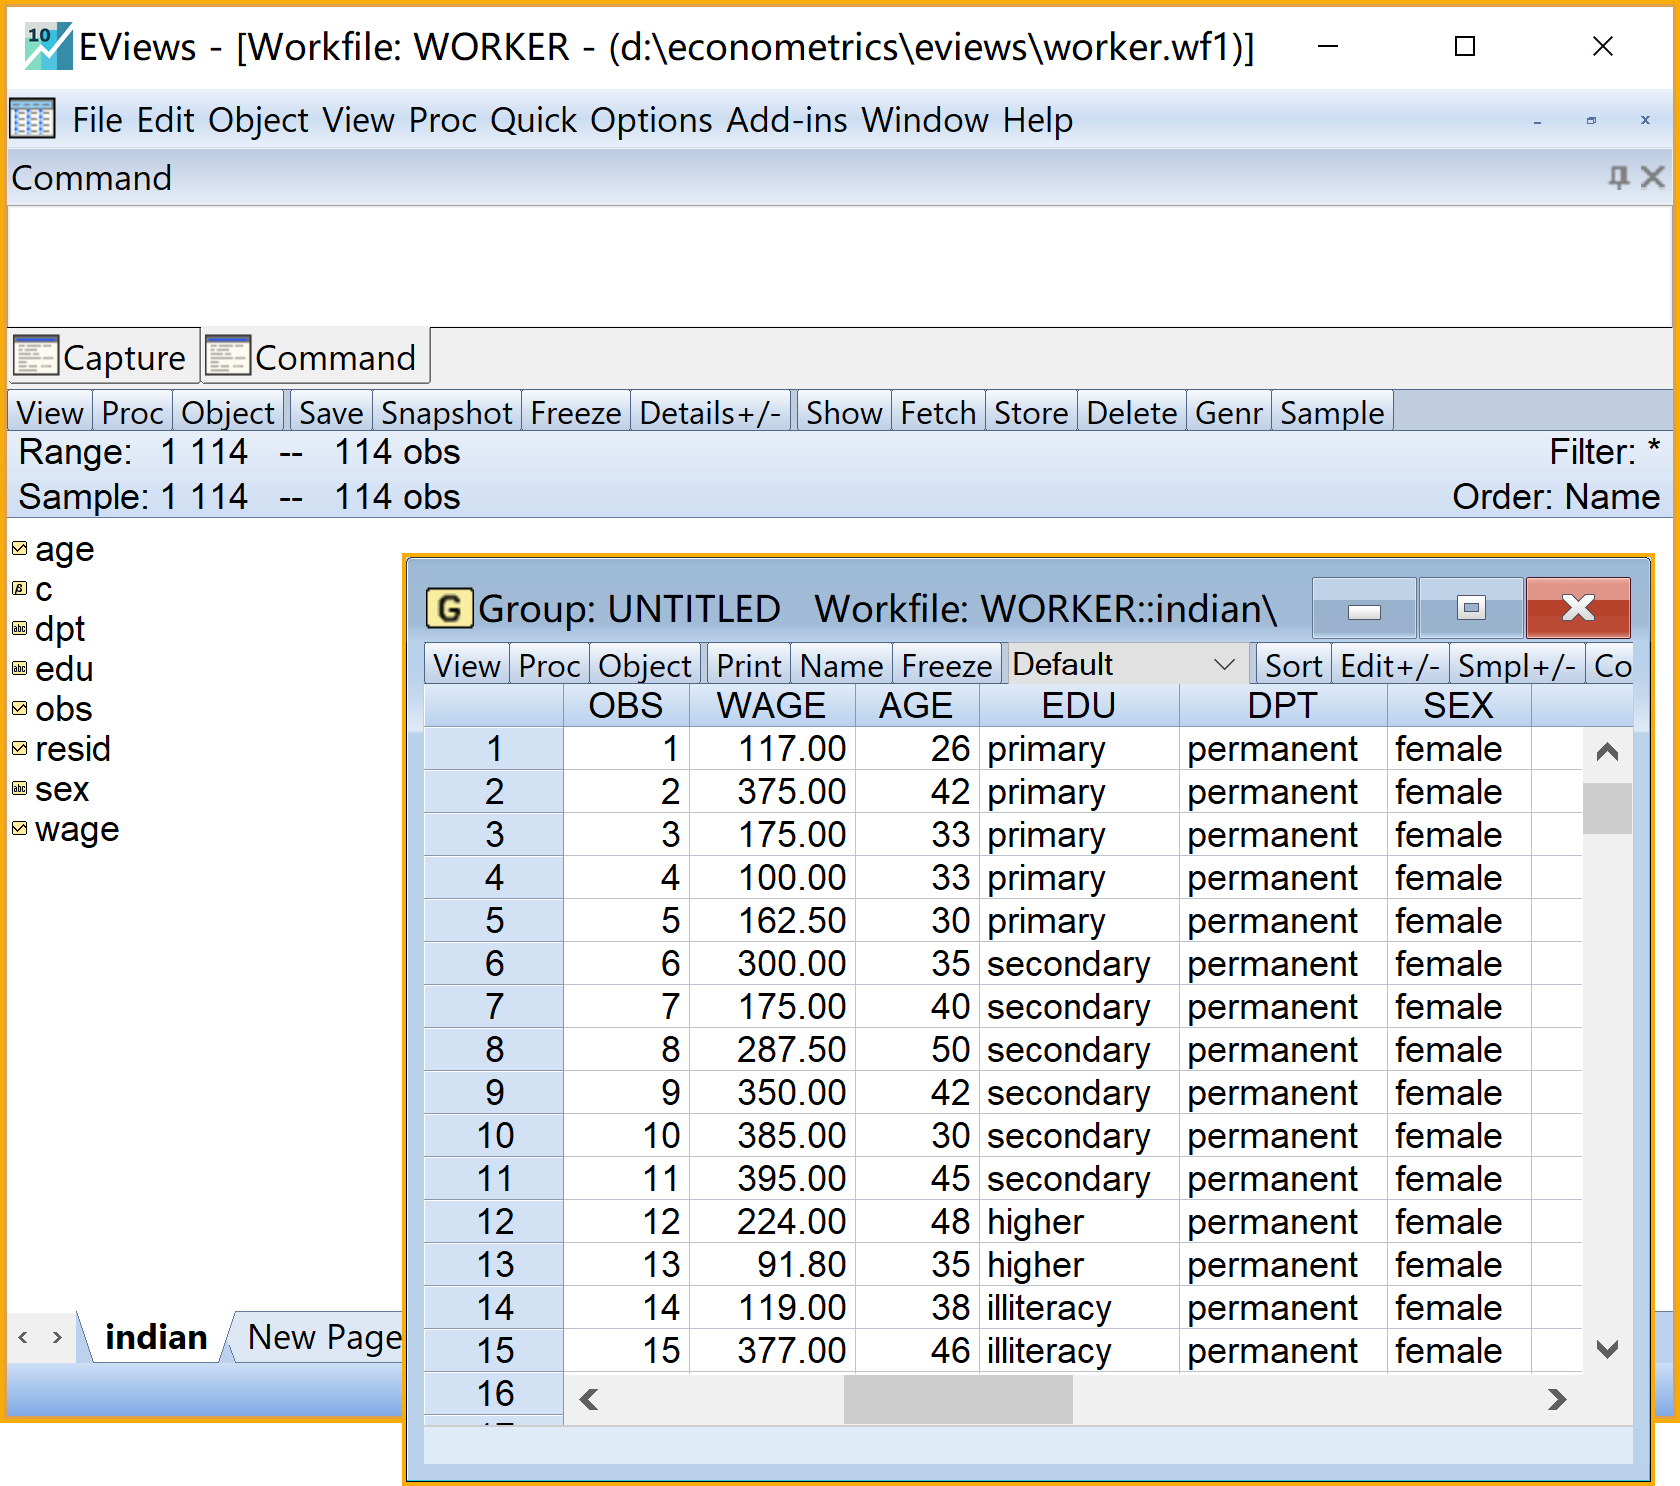
\includegraphics[width=23.33in]{picture/lab8-dummy-model/1-load-worker} 

}

\caption{导入数据的Eviews视窗}\label{fig:fig-load-worker}
\end{figure}

\subsubsection{把定性变量设置成虚拟变量体系}

\begin{itemize}
\item
  目标:学会用一套虚拟变量体系来完整表达一个定性变量
\item
  思路:按照完备、互斥的法则设置虚拟变量;如果要设置有截距模型,应统筹、优先考虑基础组的虚拟变量设置。
\item
  Eviews操作:

  \begin{enumerate}
  \def\labelenumi{\arabic{enumi})}
  \tightlist
  \item
    把定性变量\textbf{教育水平}edu(m=4)设置成虚拟变量体系。(具体操作见图\ref{fig:fig-dummy-edu})

    \begin{enumerate}
    \def\labelenumii{\alph{enumii}.}
    \tightlist
    \item
      命令视窗(Command)依次输入命令(建议分别命名为edu\_d1、edu\_d2、edu\_d3和edu\_d4)

      \begin{itemize}
      \tightlist
      \item
        \texttt{series\ edu\_d1=@recode(edu="illiteracy",1,0)\textquotesingle{}}
      \item
        \texttt{series\ edu\_d2=@recode(edu="primary",1,0)\textquotesingle{}}
      \item
        \texttt{series\ edu\_d3=@recode(edu="secondary",1,0)}
      \item
        \texttt{series\ edu\_d4=@recode(edu="higher",1,0)\textquotesingle{}}
      \end{itemize}
    \item
      运行命令:命令行中按Enter键\\
    \item
      查看结果(以组group的形式查看):

      \begin{itemize}
      \tightlist
      \item
        按住键盘Ctrl+依次点击
\includegraphics{picture/object/Series.png}\texttt{edu}、
\includegraphics{picture/object/Series.png}\texttt{edu\_d1}、
\includegraphics{picture/object/Series.png}\texttt{edu\_d2}、
\includegraphics{picture/object/Series.png}\texttt{edu\_d3}、
\includegraphics{picture/object/Series.png}\texttt{edu\_d4}
      \item
        点击鼠标右键\(\Rightarrow\) Open \(\Rightarrow\) as Group
      \end{itemize}
    \end{enumerate}
  \item
    把定性变量\textbf{合同类型}dpt(m=2)设置成虚拟变量体系。(具体操作见图\ref{fig:fig-dummy-dpt})

    \begin{enumerate}
    \def\labelenumii{\alph{enumii}.}
    \tightlist
    \item
      命令视窗(Command)依次输入命令(建议分别命名为dpt\_d1和dpt\_d2)

      \begin{itemize}
      \tightlist
      \item
        \texttt{series\ dpt\_d1=@recode(dpt="temporary",1,0)\textquotesingle{}}
      \item
        \texttt{series\ dpt\_d2=@recode(dpt="permanent",1,0)}
      \end{itemize}
    \item
      运行命令:命令行中按Enter键\\
    \item
      查看结果(以组group的形式查看):

      \begin{itemize}
      \tightlist
      \item
        按住键盘Ctrl+依次点击
\includegraphics{picture/object/Series.png}\texttt{dpt}、
\includegraphics{picture/object/Series.png}\texttt{dpt\_d1}、
\includegraphics{picture/object/Series.png}\texttt{dpt\_d2}
      \item
        点击鼠标右键\(\Rightarrow\) Open \(\Rightarrow\) as Group
      \end{itemize}
    \end{enumerate}
  \item
    把定性变量\textbf{性别}sex(m=2)设置成虚拟变量体系。(具体操作见图\ref{fig:fig-dummy-sex})

    \begin{enumerate}
    \def\labelenumii{\alph{enumii}.}
    \tightlist
    \item
      命令视窗(Command)依次输入命令(建议分别命名为sex\_d1和sex\_d2)

      \begin{itemize}
      \tightlist
      \item
        \texttt{series\ sex\_d1=@recode(sex="female",1,0)\textquotesingle{}}
      \item
        \texttt{series\ sex\_d2=@recode(sex="male",1,0)}
      \end{itemize}
    \item
      运行命令:命令行中按Enter键\\
    \item
      查看结果(以组group的形式查看):

      \begin{itemize}
      \tightlist
      \item
        按住键盘Ctrl+依次点击
\includegraphics{picture/object/Series.png}\texttt{sex}、
\includegraphics{picture/object/Series.png}\texttt{sex\_d1}、
\includegraphics{picture/object/Series.png}\texttt{sex\_d2}
      \item
        点击鼠标右键\(\Rightarrow\) Open \(\Rightarrow\) as Group
      \end{itemize}
    \end{enumerate}
  \item
    说明(\href{http://www.eviews.com/Learning/dummies.html}{Eviews代码行的解读}\^{}{[}具体细节请参看Eviews在线学习文档,网址http://www.eviews.com/Learning/dummies.html):

    \begin{enumerate}
    \def\labelenumii{\alph{enumii}.}
    \tightlist
    \item
      代码\texttt{series\ edu\_d1=@recode(edu="primary",1,0)}表示给创建一个序列(Series)对象
\includegraphics{picture/object/Series.png}\texttt{edu\_d1},并对定性变量对象
\includegraphics{picture/object/Series.png}\texttt{edu}进行重新编码处理(recode),并把重新编码处理后的数值赋值给序列(Series)对象
\includegraphics{picture/object/Series.png}\texttt{edu\_d1}。
    \item
      代码\texttt{@recode(edu="primary",1,0)}表示对定性变量对象
\includegraphics{picture/object/Series.png}\texttt{edu}进行重新编码处理。具体做法是,如果\texttt{edu}的取值为\texttt{primary},则相应赋值为1,或者就相应赋值为0。
    \end{enumerate}
  \end{enumerate}
\end{itemize}

\begin{figure}

{\centering 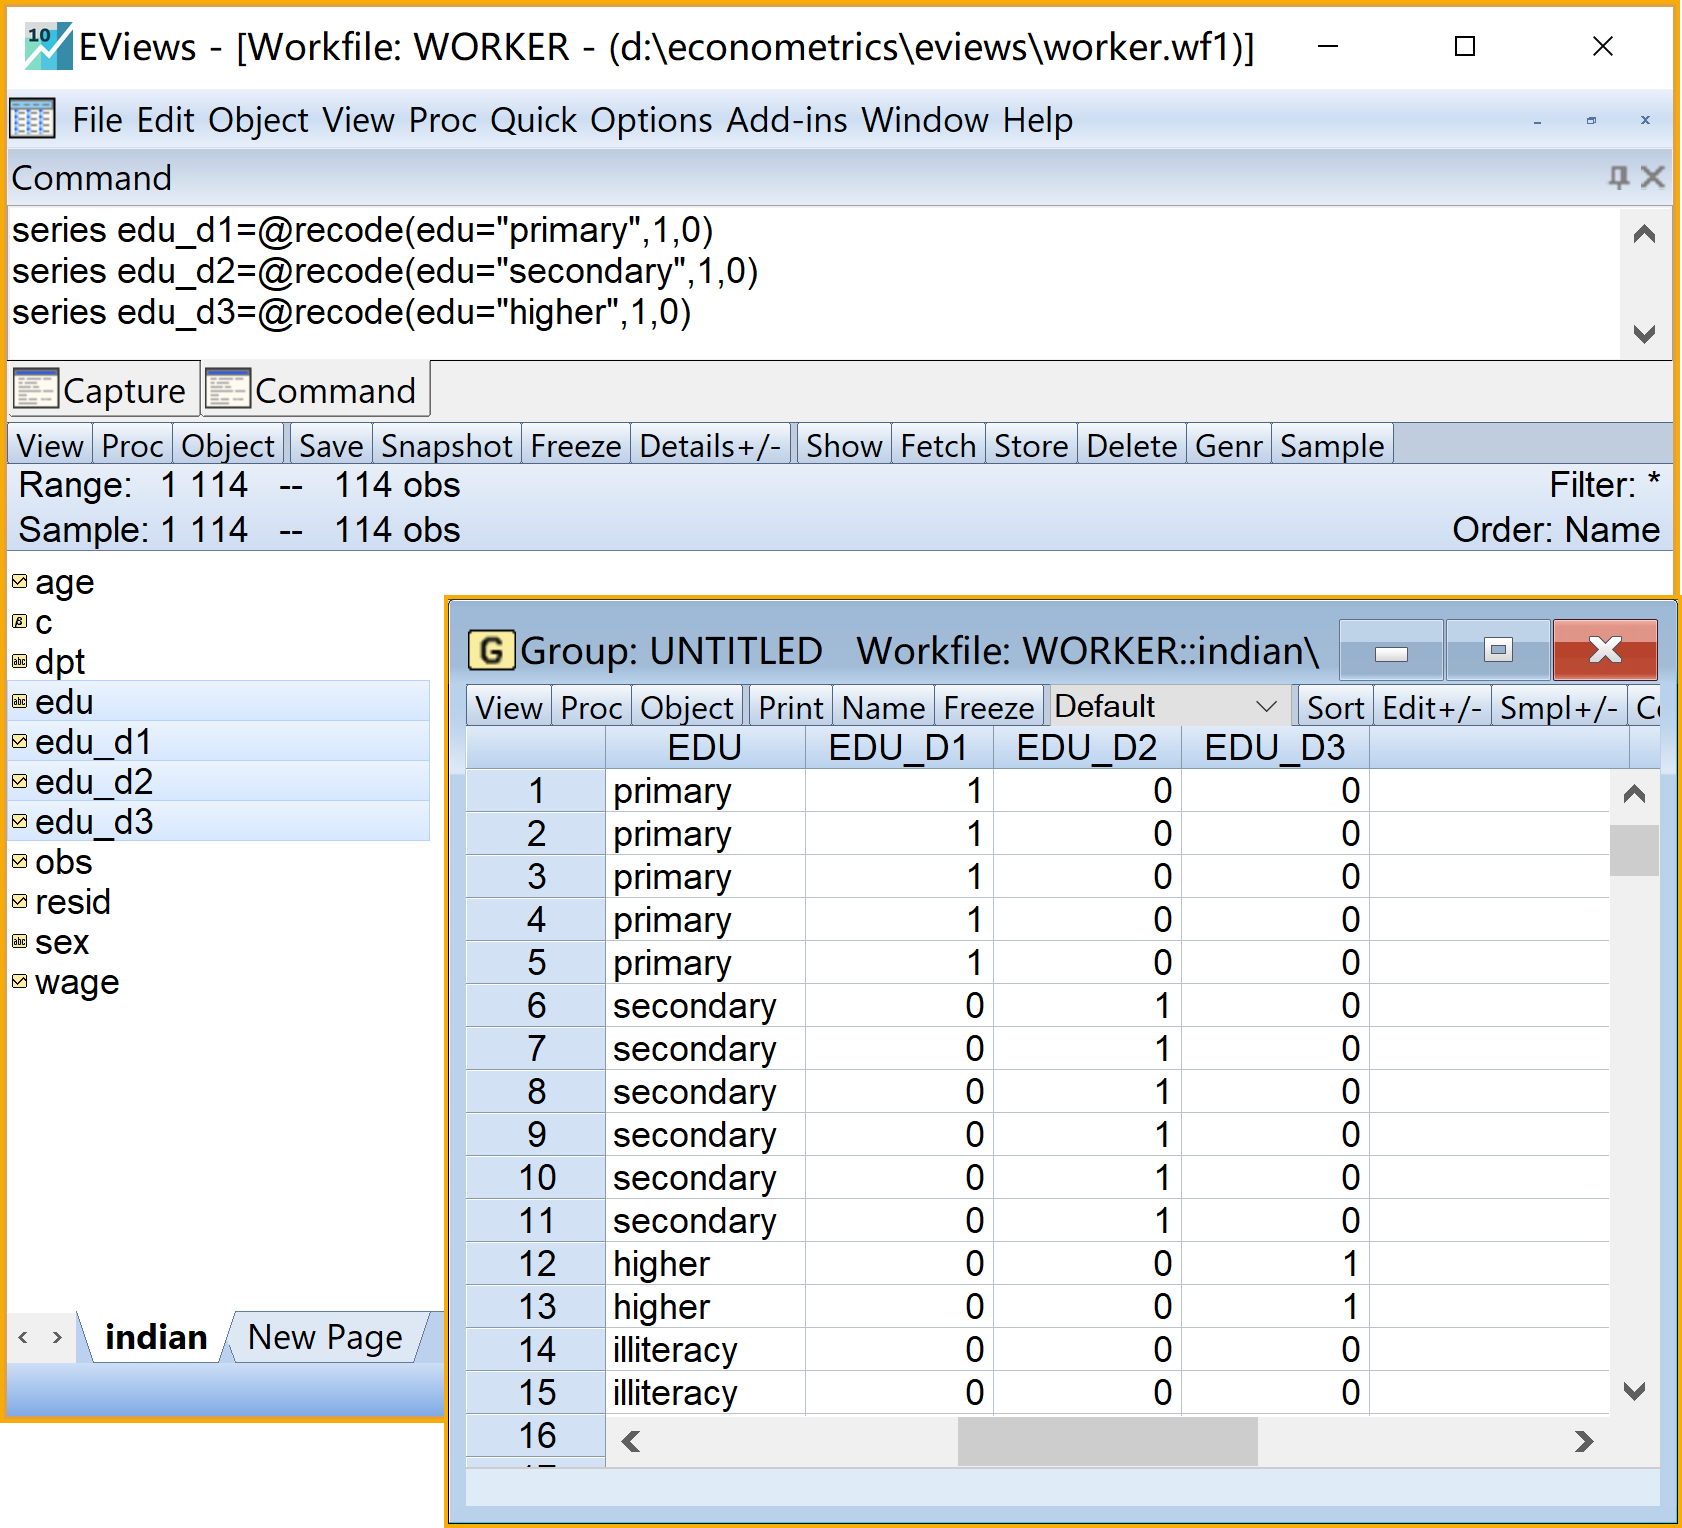
\includegraphics[width=23.36in]{picture/lab8-dummy-model/1-dummy-edu} 

}

\caption{定性变量edu用虚拟变量体系表达}\label{fig:fig-dummy-edu}
\end{figure}

\begin{figure}

{\centering 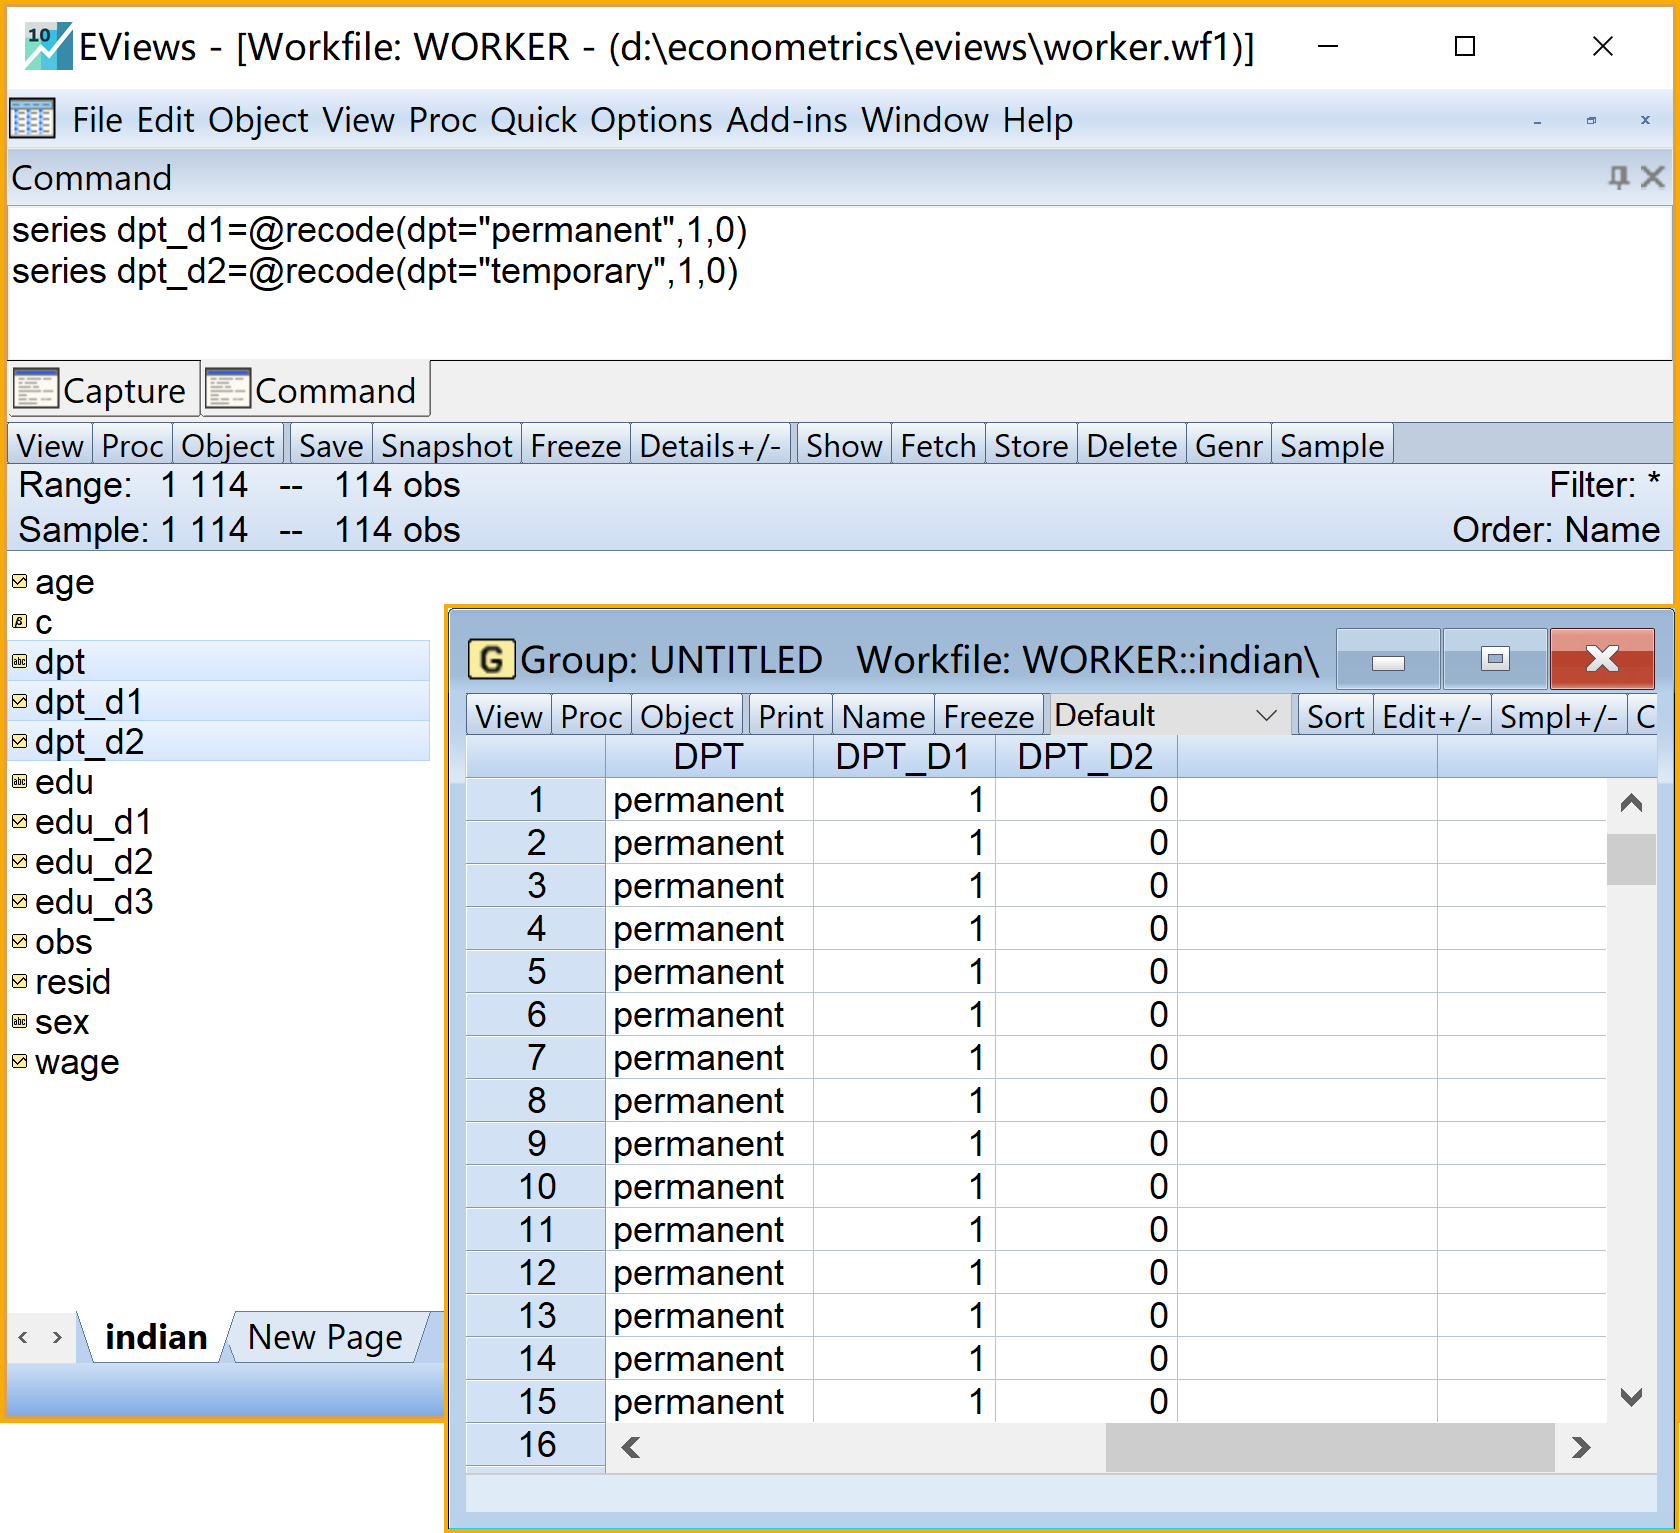
\includegraphics[width=23.33in]{picture/lab8-dummy-model/1-dummy-dpt} 

}

\caption{定性变量dpt用虚拟变量体系表达}\label{fig:fig-dummy-dpt}
\end{figure}

\begin{figure}

{\centering 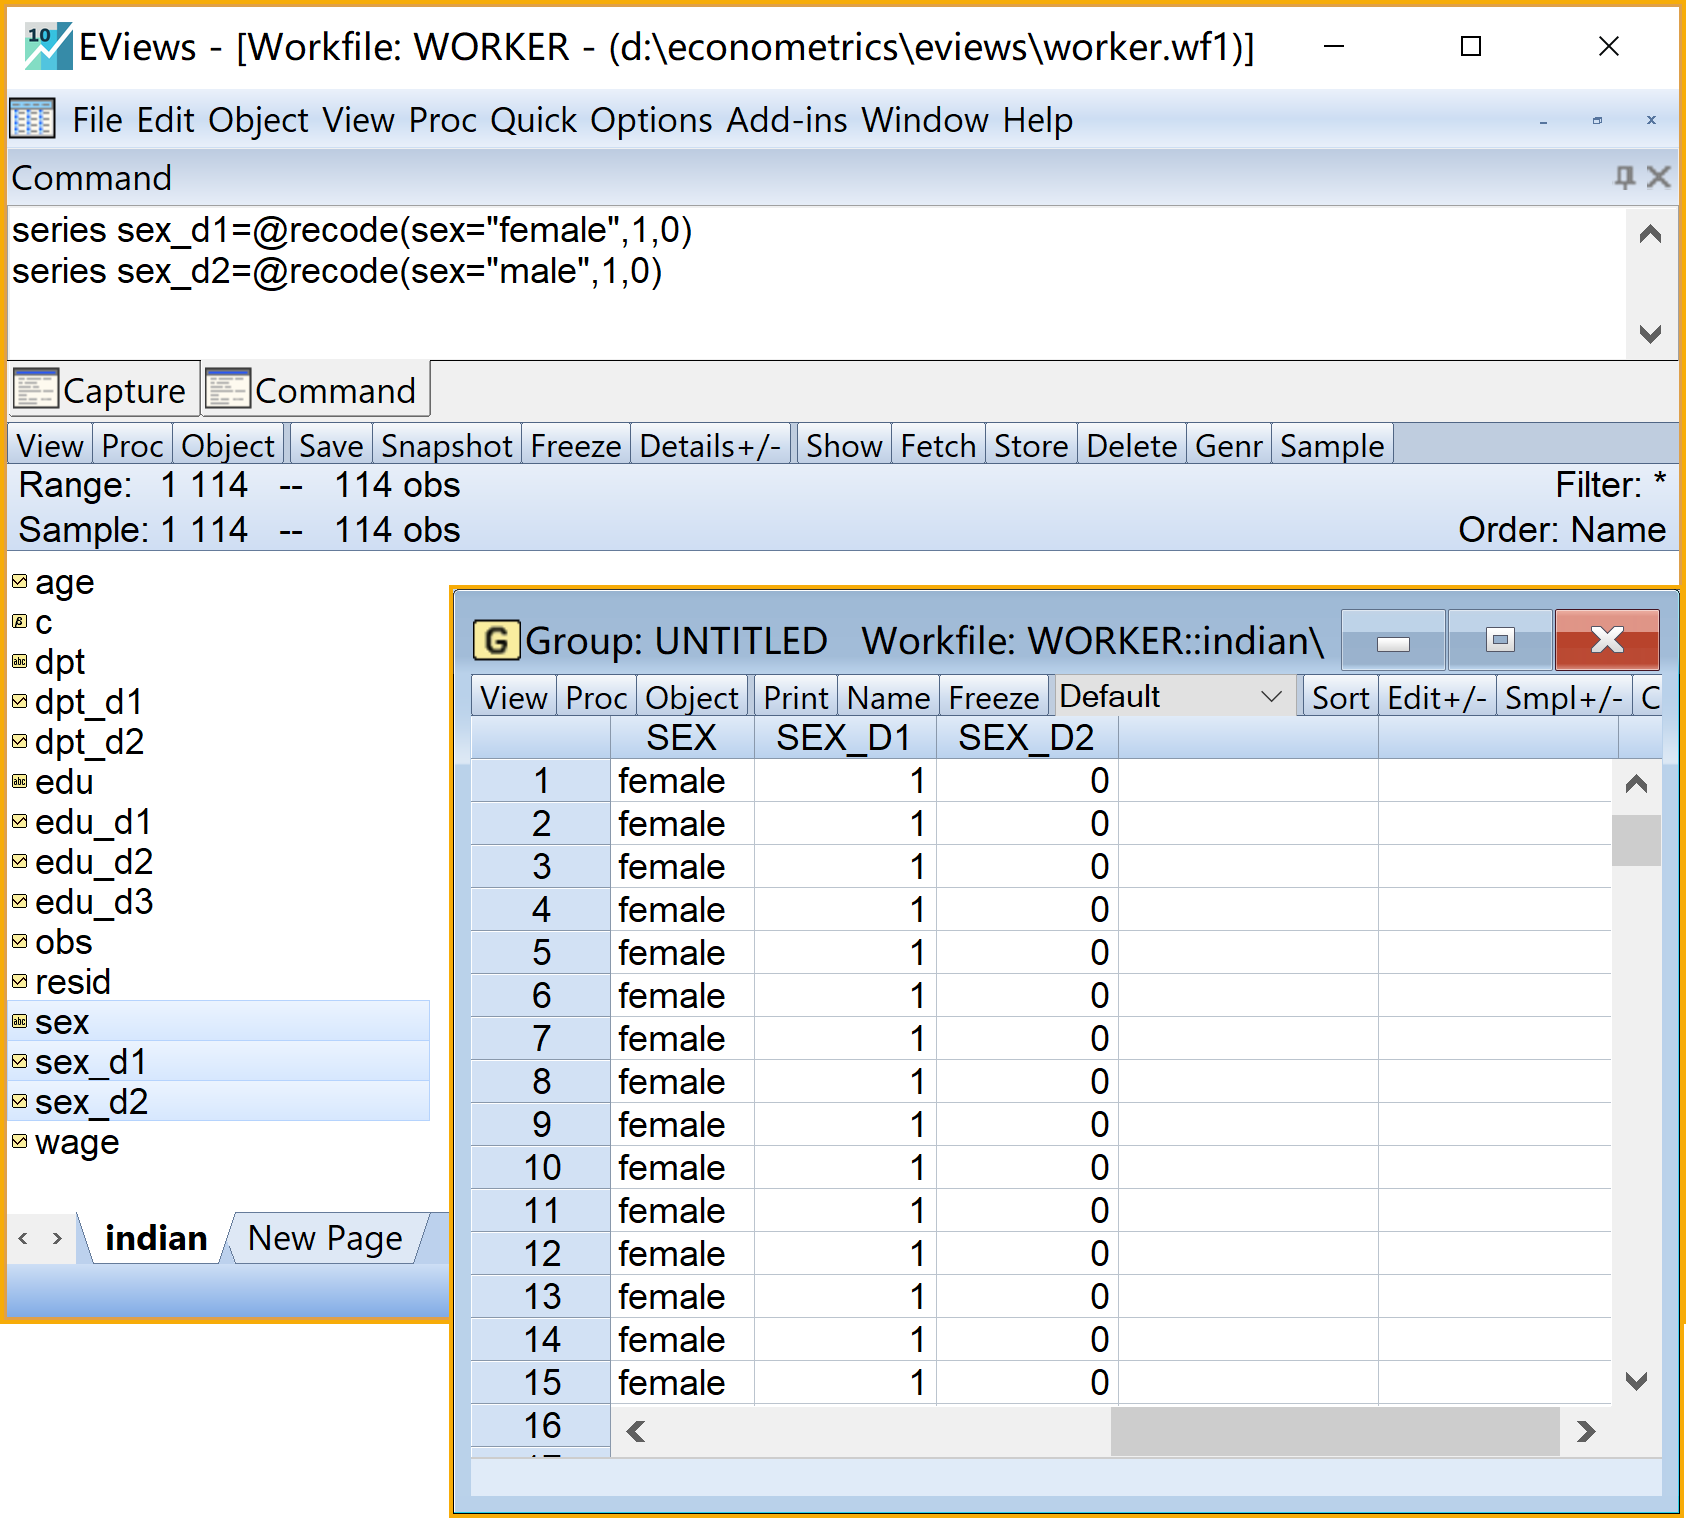
\includegraphics[width=23.42in]{picture/lab8-dummy-model/1-dummy-sex} 

}

\caption{定性变量sex用虚拟变量体系表达}\label{fig:fig-dummy-sex}
\end{figure}

\paragraph{操作解读}

\begin{verbatim}
## Loading required package: psych
\end{verbatim}

实际操作中,我们首先要对定性变量进行重新编码,设置成各自的虚拟变量体系。Eviews中对定性变量重新编码为虚拟变量的代码函数为\texttt{@recode()}。我们可以事先将一个定性变量\textbf{完全地}进行虚拟变量编码\footnote{此时我们可以完全不用关心模型是否有截距(意味着是否有对照比较的\textbf{基础组})}。也就是说,如果一个定性变量有m个属性,我们可以直接设置m个虚拟变量。

此外,便于后续多个模型的分析甄选,我们还应该进一步统一设计虚拟变量的名称、命名的顺序等。例如,假设后续的备选模型中将基础组设定为\{文盲,临时工,女性\}(也即\{illiteracy,temporary,female\})\footnote{理论上,基础组如何选择并不会从根本上改变模型的实际经济学意义,只是一旦选定一个基础组,也就意味着确定了一个相互比较的``基础参照系''。}。则可以将全部定性变量的基础组属性\{illiteracy,temporary,female\}分别设置为虚拟变量\texttt{edu\_D1}(见表\ref{tab:tab-edu})、\texttt{dpt\_D1}和\texttt{sex\_D1}(见表\ref{tab:tab-dpt-sex})。

\begin{table}

\caption{\label{tab:tab-edu}用虚拟变量系统完全表达定性变量edu}
\centering
\begin{tabular}[t]{llrrrr}
\toprule
  & edu & edu\_D1 & edu\_D2 & edu\_D3 & edu\_D4\\
\midrule
1 & primary & 0 & 1 & 0 & 0\\
2 & primary & 0 & 1 & 0 & 0\\
6 & secondary & 0 & 0 & 1 & 0\\
7 & secondary & 0 & 0 & 1 & 0\\
12 & higher & 0 & 0 & 0 & 1\\
\addlinespace
13 & higher & 0 & 0 & 0 & 1\\
14 & illiteracy & 1 & 0 & 0 & 0\\
15 & illiteracy & 1 & 0 & 0 & 0\\
\bottomrule
\end{tabular}
\end{table}

\begin{table}
\caption{\label{tab:tab-dpt-sex}用虚拟变量系统分别完全表达定性变量dpt和sex}

\centering
\begin{tabular}[t]{llrr}
\toprule
  & dpt & dpt\_D1 & dpt\_D2\\
\midrule
1 & permanent & 0 & 1\\
2 & permanent & 0 & 1\\
3 & permanent & 0 & 1\\
112 & temporary & 1 & 0\\
113 & temporary & 1 & 0\\
114 & temporary & 1 & 0\\
\bottomrule
\end{tabular}
\centering
\begin{tabular}[t]{llrr}
\toprule
  & sex & sex\_D1 & sex\_D2\\
\midrule
1 & female & 1 & 0\\
2 & female & 1 & 0\\
3 & female & 1 & 0\\
112 & male & 0 & 1\\
113 & male & 0 & 1\\
114 & male & 0 & 1\\
\bottomrule
\end{tabular}
\end{table}

\hypertarget{group1}{%
\subsubsection{只含有虚拟变量的回归模型(考虑基础组的情形)}\label{group1}}

\paragraph{加法模型}

\begin{itemize}
\item
  目标:把定性变量的虚拟变量以独立项的形式引入模型方程,解释回归报告
\item
  思路:确定\textbf{基础组},设置总体回归模型(PRM),进行OLS估计,得到Eviews分析报告
\item
  理论提示:

  \begin{itemize}
  \tightlist
  \item
    模型1:只含有虚拟变量的、加法形式的\textbf{经典回归模型}见方程\eqref{eq:only-plus}
  \item
    模型2:只含有虚拟变量的、加法形式的\textbf{半对数回归模型}见方程\eqref{eq:only-plus-log}
  \end{itemize}
\end{itemize}

\begin{align}
wage_i & =\alpha_1+\alpha_2edu_{D2,i}+\alpha_3edu_{D3,i}+\alpha_4edu_{D4,i}+\beta_2 dpt_{D2,i}+\gamma_2 sex_{D2,i}+u_i  \label{eq:only-plus} \\
ln(wage_i) & =\alpha_1+\alpha_2edu_{D2,i}+\alpha_3edu_{D3,i}+\alpha_4edu_{D4,i}+\beta_2 dpt_{D2,i}+\gamma_2 
sex_{D2,i}+u_i  \label{eq:only-plus-log}\\
\end{align}

\begin{itemize}
\tightlist
\item
  Eviews操作1(只含有虚拟变量的、加法形式的\textbf{经典回归模型}见方程\eqref{eq:only-plus},菜单操作实现具体见图\ref{fig:only-plus}):

  \begin{enumerate}
  \def\labelenumi{\arabic{enumi})}
  \tightlist
  \item
    确定参照组为{[}\textbf{文盲\&短期合同\&女性}{]},则如下虚拟变量将\textbf{不进入}回归模型

    \begin{enumerate}
    \def\labelenumii{\alph{enumii}.}
    \tightlist
    \item
      
\includegraphics{picture/object/Series.png}\texttt{edu\_d1}
    \item
      
\includegraphics{picture/object/Series.png}\texttt{dpt\_d1}
    \item
      
\includegraphics{picture/object/Series.png}\texttt{sex\_d1}
    \end{enumerate}
  \item
    设置回归模型。进入引导设置Equation Estimation \(\Rightarrow\)
    specification

    \begin{enumerate}
    \def\labelenumii{\alph{enumii}.}
    \tightlist
    \item
      Equation
      specification:输入命令\texttt{wage\ c\ edu\_d2\ edu\_d3\ edu\_d4\ dpt\_d2\ sex\_d2}
    \item
      Estimation settings:

      \begin{itemize}
      \tightlist
      \item
        Method: 下拉选择LS - Least Squares (NLS and ARMA)
      \item
        Sample: (默认设置)
      \end{itemize}
    \item
      点击完成:OK
    \item
      命名保存方程对象
\includegraphics{picture/object/Equation.png}:(建议命名为\texttt{eq\_only\_plus})
    \item
      查看结果:双击
\includegraphics{picture/object/Equation.png}\texttt{eq\_only\_plus}
    \end{enumerate}
  \end{enumerate}
\end{itemize}

具体Eviews报告见\ref{fig:only-plus-report}:

\begin{figure}

{\centering 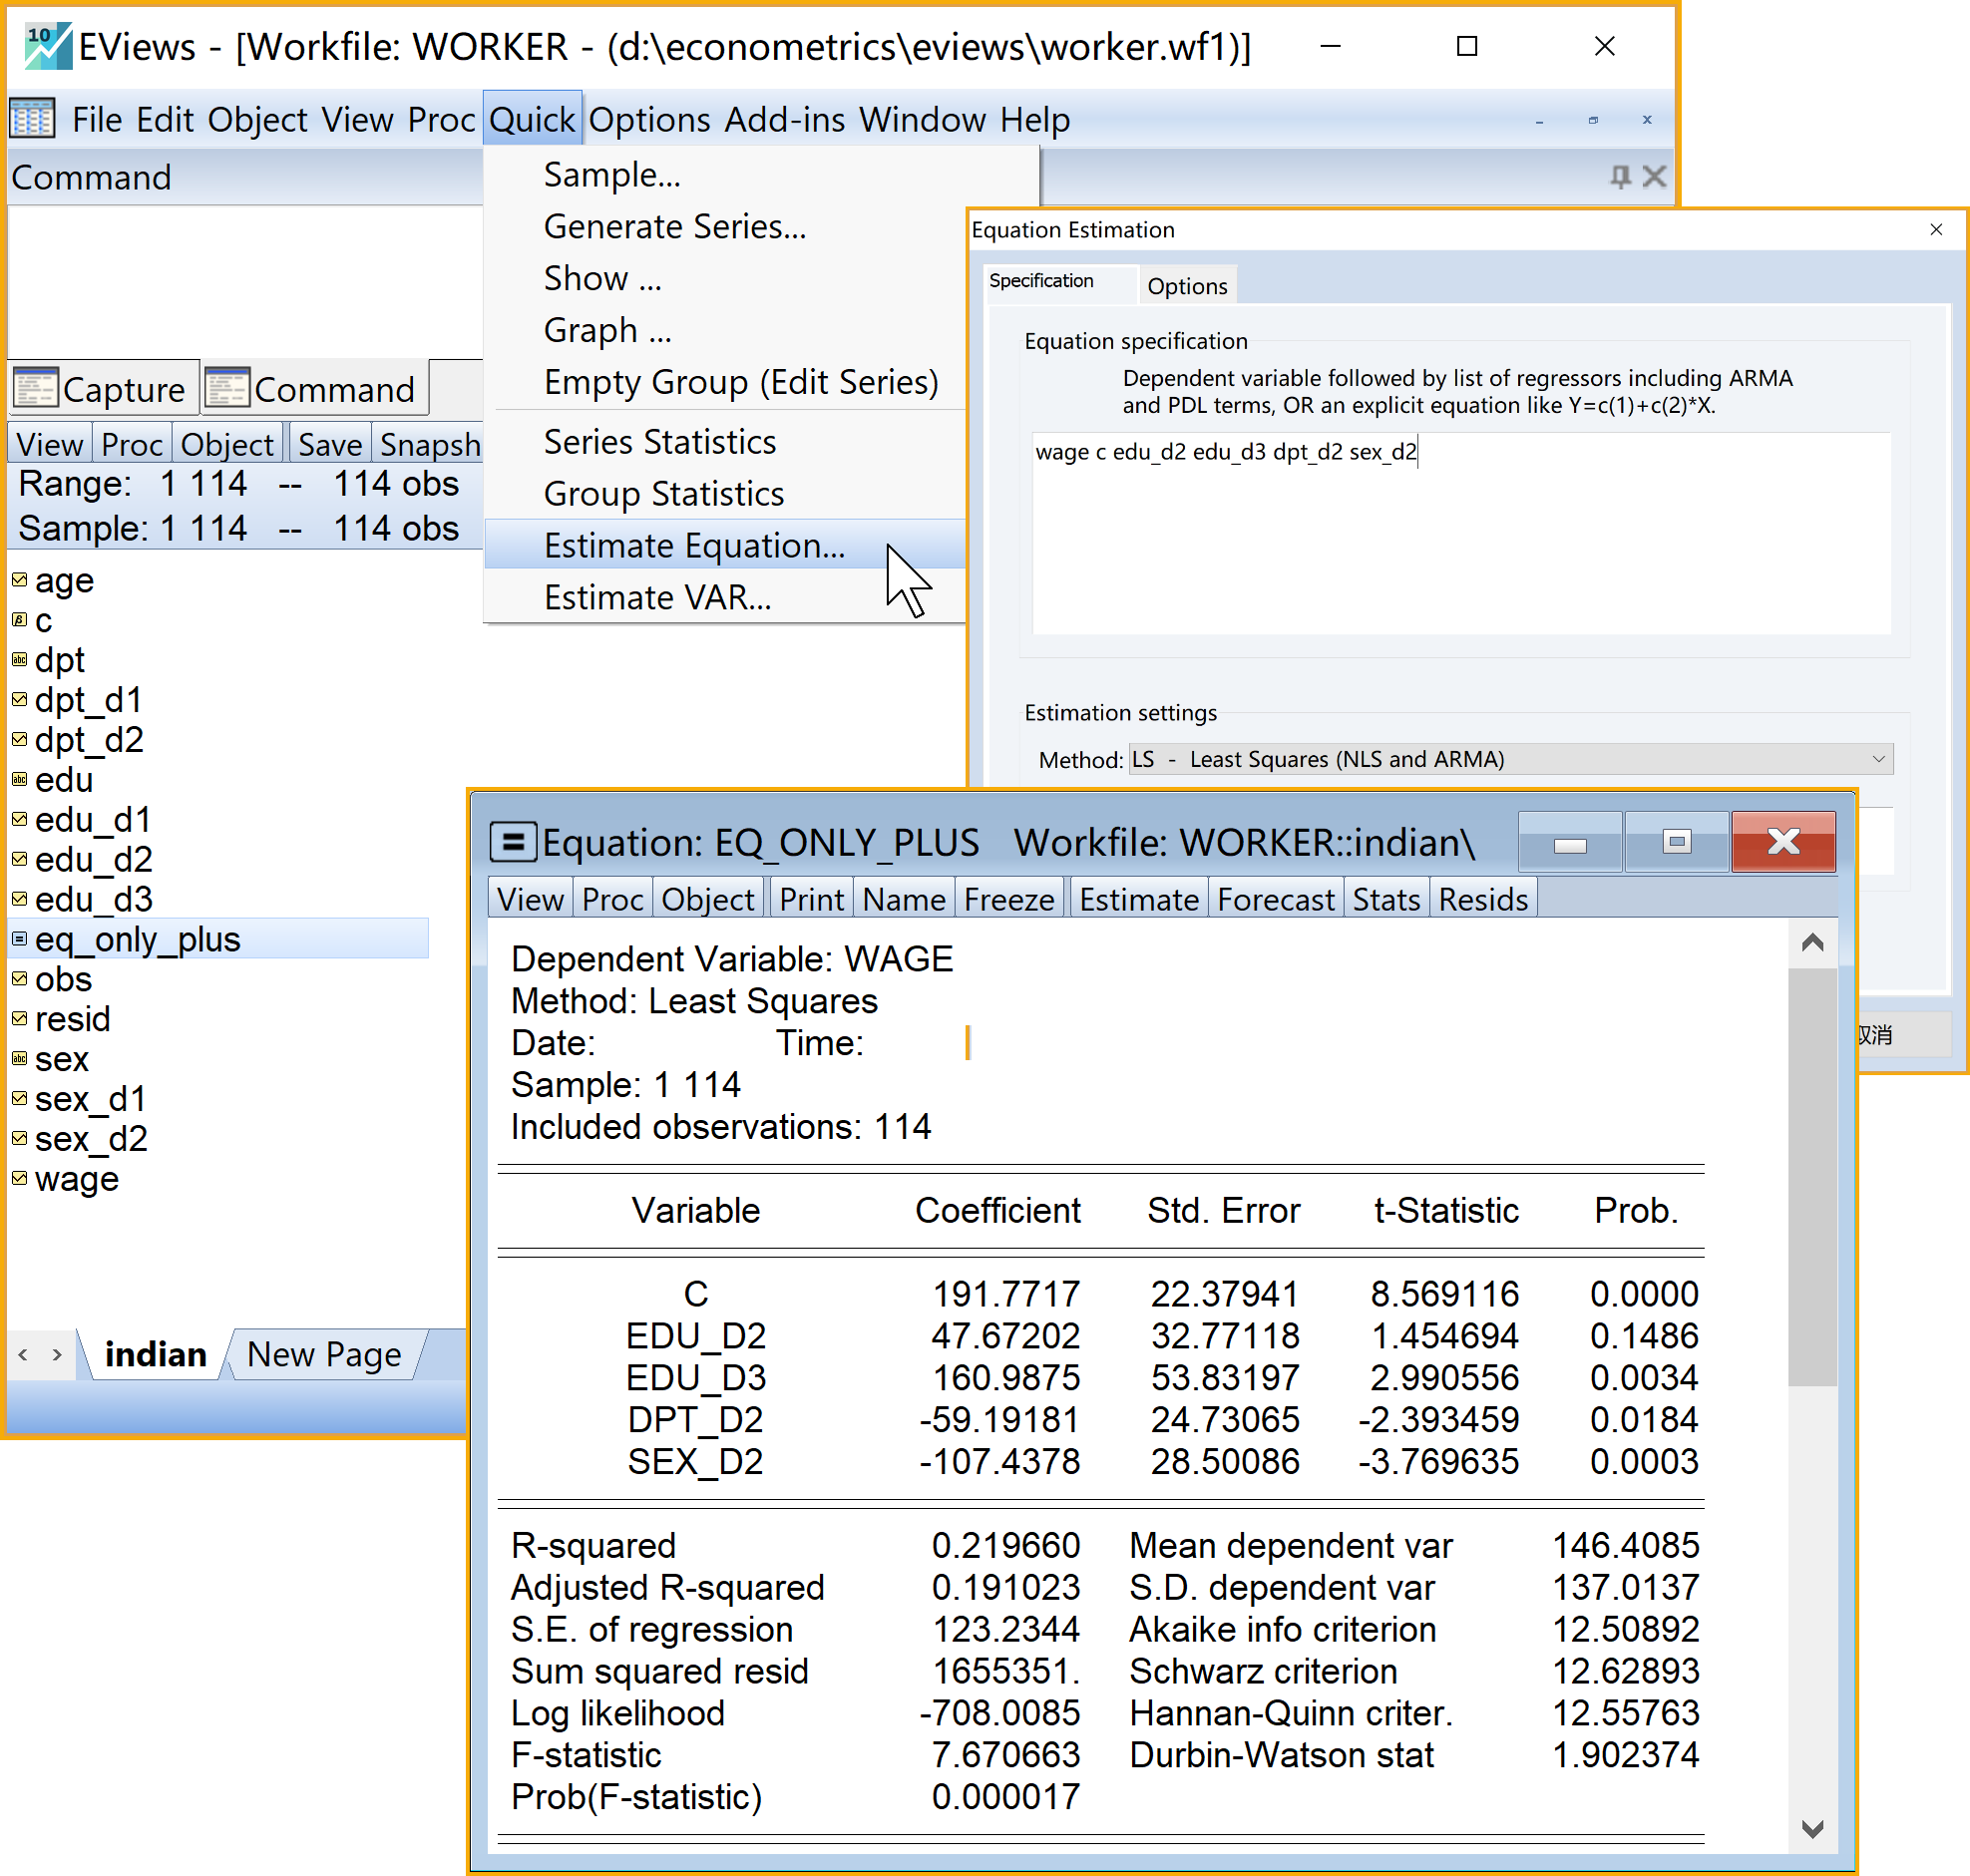
\includegraphics[width=27.43in]{picture/lab8-dummy-model/2-only-plus} 

}

\caption{只含虚拟变量的、加法形式的经典线性回归模型Eviews实现}\label{fig:only-plus}
\end{figure}

\begin{figure}

{\centering 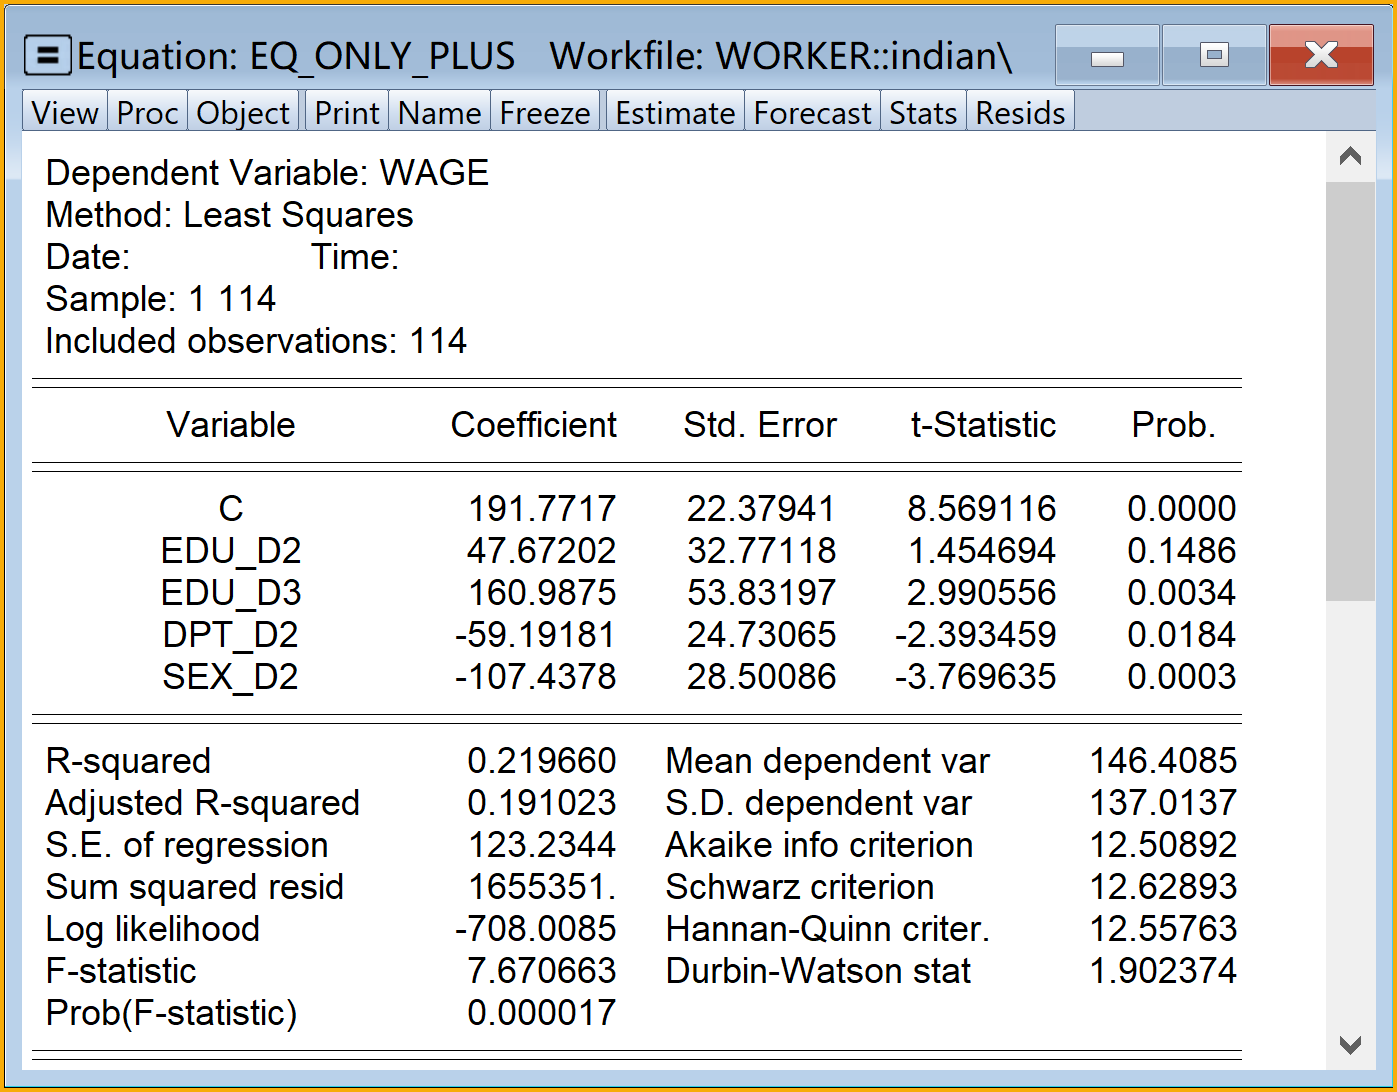
\includegraphics[width=19.4in]{picture/lab8-dummy-model/2-only-plus-report} 

}

\caption{只含虚拟变量的、加法形式的经典线性回归模型Eviews报告}\label{fig:only-plus-report}
\end{figure}

\begin{itemize}
\tightlist
\item
  Eviews操作2(只含有虚拟变量的、加法形式的\textbf{半对数回归模型}见方程\eqref{eq:only-plus-log},菜单操作实现具体见图\ref{fig:only-plus-log}):

  \begin{enumerate}
  \def\labelenumi{\arabic{enumi})}
  \tightlist
  \item
    确定参照组为{[}\textbf{文盲\&短期合同\&女性}{]},则如下虚拟变量将\textbf{不进入}回归模型

    \begin{enumerate}
    \def\labelenumii{\alph{enumii}.}
    \tightlist
    \item
      
\includegraphics{picture/object/Series.png}\texttt{edu\_d1}
    \item
      
\includegraphics{picture/object/Series.png}\texttt{dpt\_d1}
    \item
      
\includegraphics{picture/object/Series.png}\texttt{sex\_d1}
    \end{enumerate}
  \item
    设置回归模型。进入引导设置Equation Estimation \(\Rightarrow\)
    specification

    \begin{enumerate}
    \def\labelenumii{\alph{enumii}.}
    \tightlist
    \item
      Equation
      specification:输入命令\texttt{log(wage)\ c\ edu\_d2\ edu\_d3\ edu\_d4\ dpt\_d2\ sex\_d2}
    \item
      Estimation settings:

      \begin{itemize}
      \tightlist
      \item
        Method: 下拉选择LS - Least Squares (NLS and ARMA)
      \item
        Sample: (默认设置)
      \end{itemize}
    \item
      点击完成:OK
    \item
      命名保存方程对象
\includegraphics{picture/object/Equation.png}:(建议命名为\texttt{eq\_only\_plus\_log})
    \item
      查看结果:双击
\includegraphics{picture/object/Equation.png}\texttt{eq\_only\_plus\_log}
    \end{enumerate}
  \end{enumerate}
\end{itemize}

具体Eviews报告见\ref{fig:only-plus-log-report}:

\begin{figure}

{\centering 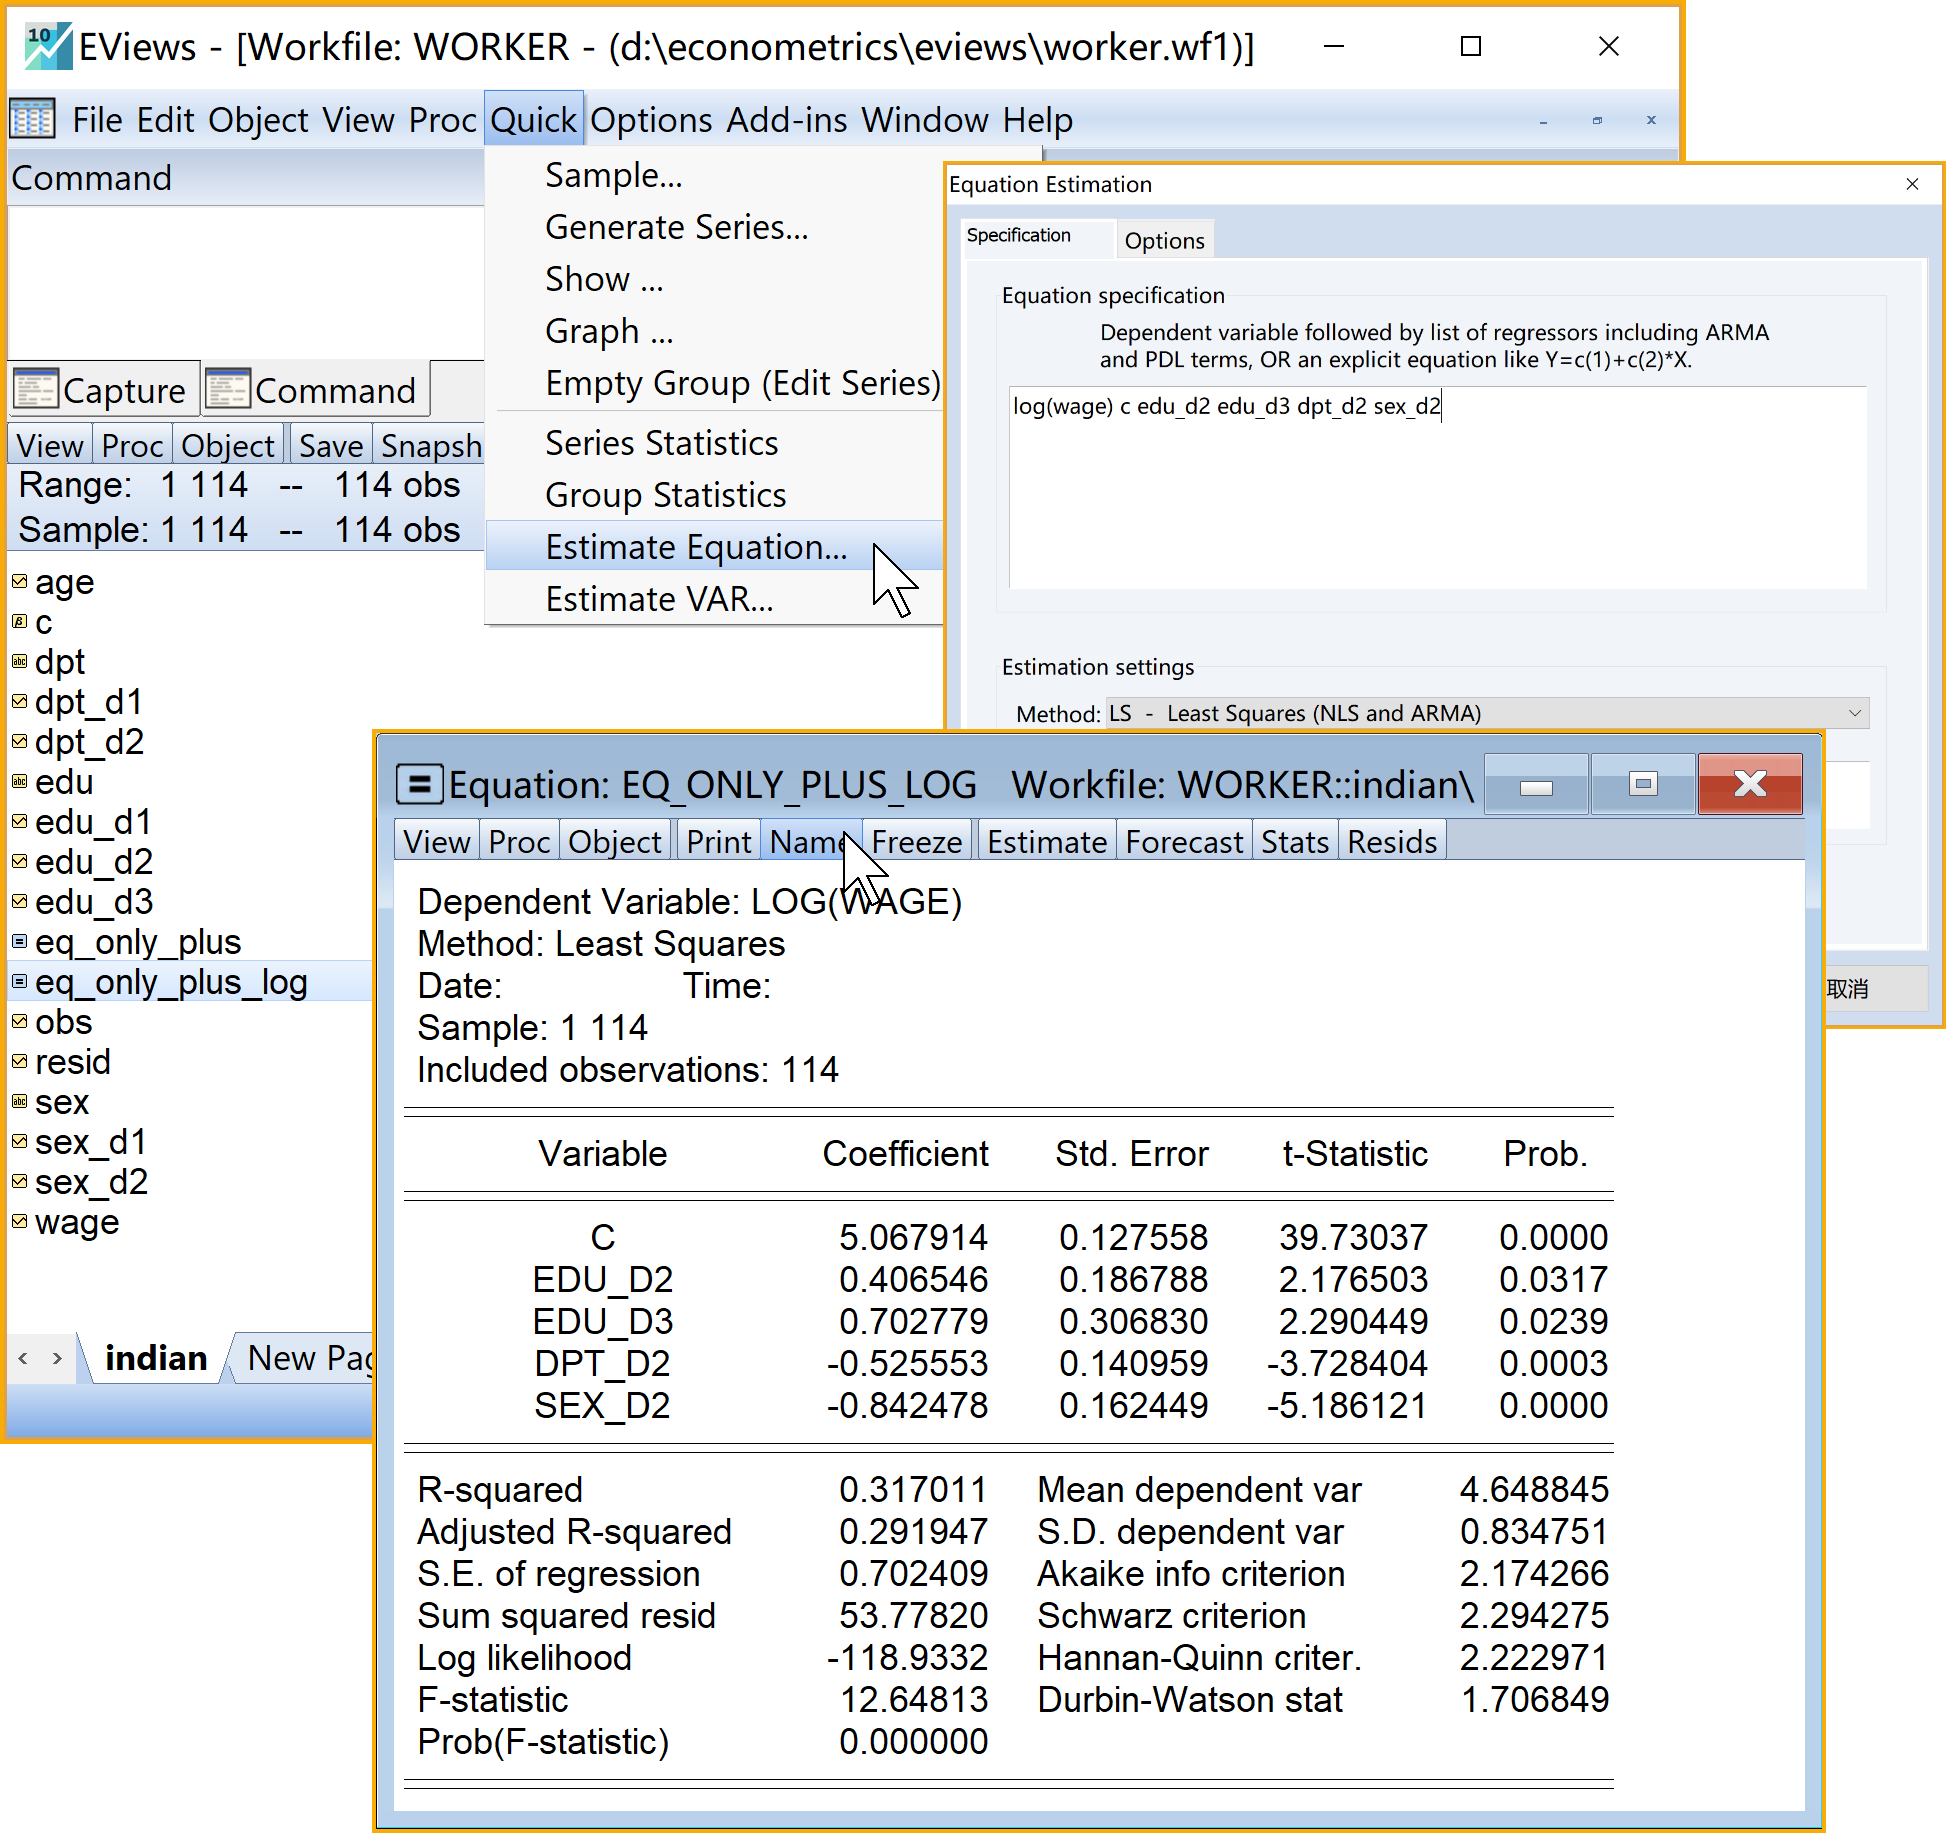
\includegraphics[width=27.03in]{picture/lab8-dummy-model/2-only-plus-log} 

}

\caption{只含虚拟变量的、加法形式的半对数线性回归模型Eviews实现}\label{fig:only-plus-log}
\end{figure}

\begin{figure}

{\centering 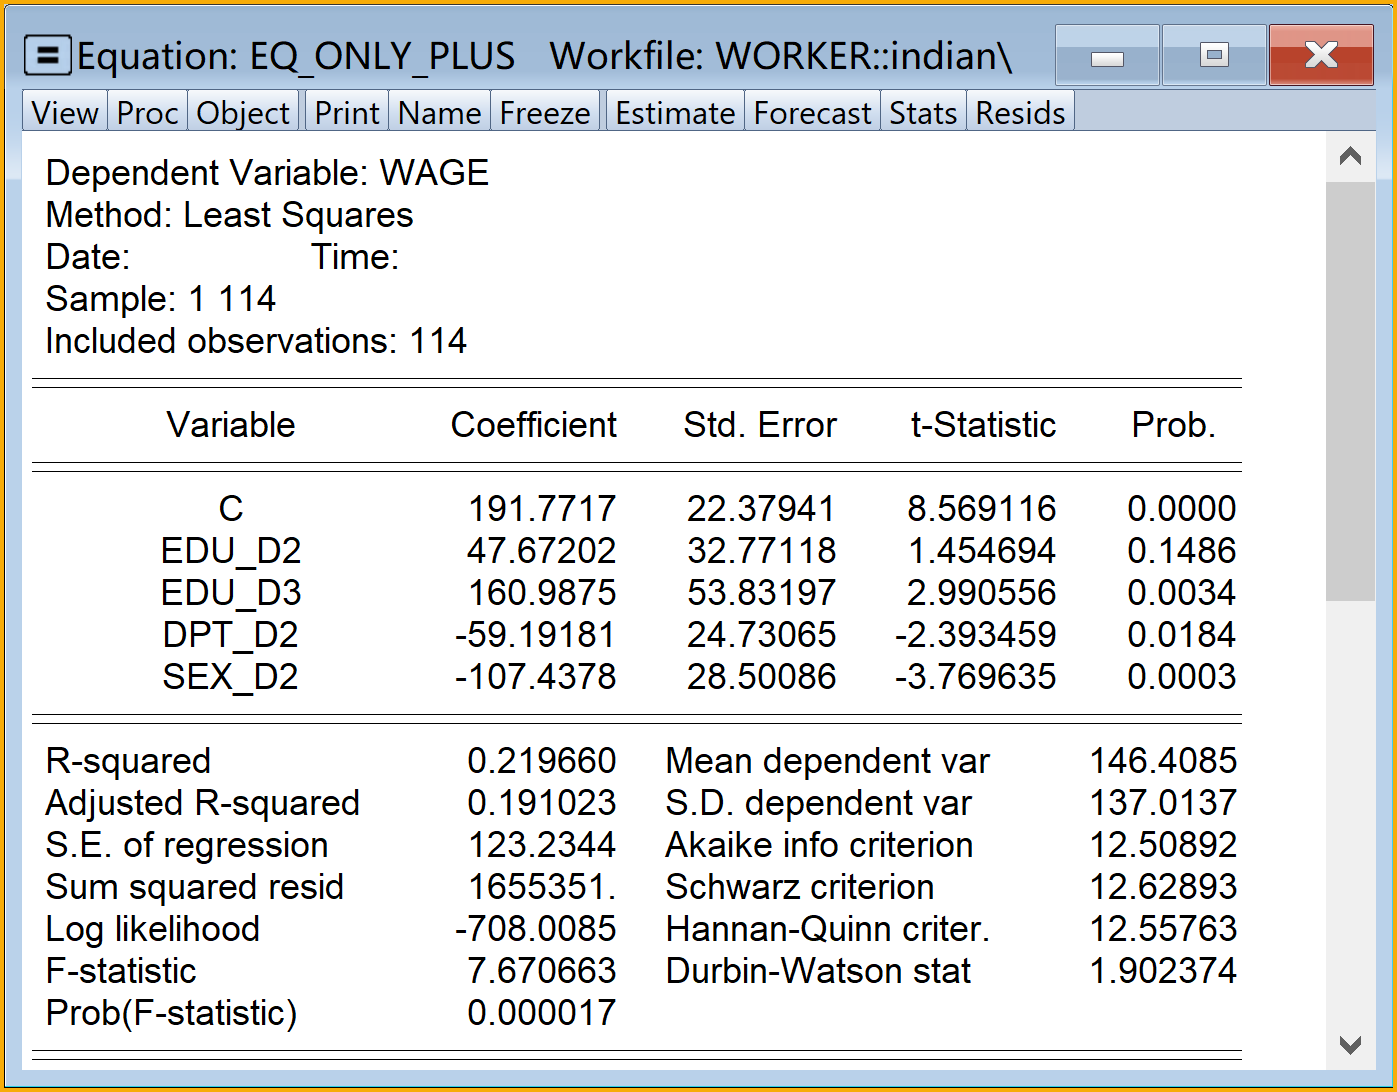
\includegraphics[width=19.4in]{picture/lab8-dummy-model/2-only-plus-report} 

}

\caption{只含虚拟变量的、加法形式的半对数线性回归模型Eviews报告}\label{fig:only-plus-log-report}
\end{figure}

\subparagraph{报告解读}

只含虚拟变量的、加法形式的经典回归模型Eviews结果简要报告如下:

\textbackslash{}begin\{alignedat\}\{5\} \&
\widehat{wage}=+\&130.36+\&10.47edu\_D2+\&49.71edu\_D3+\&162.59edu\_D4+\&59.37dpt\_D2
\textbackslash{} \&
\text{(t)}\&(7.3397)\&(0.3126)\&(1.4818)\&(2.9944)\&(2.3899)
\textbackslash{} \&
\text{(se)}\&(17.7609)\&(33.4850)\&(33.5470)\&(54.2989)\&(24.8399)
\textbackslash{} \& \quad-\&106.49sex\_D2 \textbackslash{} \&
\text{(t)}\&(-3.7005) \textbackslash{} \& \text{(se)}\&(28.7784)
\textbackslash{} \& \text{(fitness)}\& \quad\& R\^{}2=0.2204\&
\bar\{R\^{}2\}=0.1843\& F\^{}\{\ast\}=6.1053
\textbackslash{}end\{alignedat\}

只含虚拟变量的、加法形式的半对数回归模型Eviews结果简要报告如下:

\textbackslash{}begin\{alignedat\}\{5\} \&
\widehat{log(wage)}=+\&4.53+\&0.06edu\_D2+\&0.42edu\_D3+\&0.71edu\_D4+\&0.53dpt\_D2
\textbackslash{} \&
\text{(t)}\&(44.7474)\&(0.3045)\&(2.1853)\&(2.2995)\&(3.7187)
\textbackslash{} \&
\text{(se)}\&(0.1012)\&(0.1909)\&(0.1912)\&(0.3095)\&(0.1416)
\textbackslash{} \& \quad-\&0.84sex\_D2 \textbackslash{} \&
\text{(t)}\&(-5.1040) \textbackslash{} \& \text{(se)}\&(0.1640)
\textbackslash{} \& \text{(fitness)}\& \quad\& R\^{}2=0.3176\&
\bar\{R\^{}2\}=0.2860\& F\^{}\{\ast\}=10.0528
\textbackslash{}end\{alignedat\}

\paragraph{乘法模型}

\begin{itemize}
\item
  目标:把定性变量的虚拟变量以交叉项的形式引入模型方程,解释回归报告
\item
  思路:确定\textbf{基础组},设置总体回归模型(PRM),进行OLS估计,得到Eviews分析报告
\item
  理论提示:

  \begin{itemize}
  \tightlist
  \item
    模型1:只含有虚拟变量的、乘法形式的\textbf{经典回归模型}见方程\eqref{eq:only-prod}和方程\eqref{eq:only-prod-part};
  \item
    模型2:只含有虚拟变量的、乘法形式的\textbf{半对数回归模型}见方程\eqref{eq:only-prod-log-part}
  \end{itemize}
\end{itemize}

\[\begin{equation}
\begin{split}
wage_i & =\alpha_1+\alpha_2edu_{D2,i}+\alpha_3edu_{D3,i}+\alpha_4edu_{D4,i}+\beta_2 dpt_{D2,i}+\gamma_2sex_{D2,i}
\\ & +\lambda_2edu_{D2,i} \ast dpt_{D2,i}+\lambda_3edu_{D3,i}\ast dpt_{D2,i} +\lambda_4edu_{D4,i}\ast dpt_{D2,i}+u_i  
\end{split}
\label{eq:only-prod} 
\end{equation}\]

\begin{align}
\begin{split}
wage_i & =\alpha_1+\beta_2 dpt_{D2,i}+\gamma_2sex_{D2,i}  \\
& +\lambda_2edu_{D2,i} \ast dpt_{D2,i}+\lambda_3edu_{D3,i}\ast dpt_{D2,i} +\lambda_4edu_{D4,i}\ast dpt_{D2,i}+u_i 
\end{split}
\label{eq:only-prod-part} 
\end{align}

\begin{align}
\begin{split}
ln(wage_i) & =\alpha_1+\beta_2 dpt_{D2,i}+\gamma_2sex_{D2,i} \\
& +\lambda_2edu_{D2,i} \ast dpt_{D2,i}+\lambda_3edu_{D3,i}\ast dpt_{D2,i}+\lambda_4edu_{D4,i}\ast dpt_{D2,i} +u_i 
\end{split}
\label{eq:only-prod-log-part} 
\end{align}

\begin{itemize}
\tightlist
\item
  Eviews操作1(只含有虚拟变量的、乘法形式的\textbf{经典回归模型}见方程\eqref{eq:only-prod},菜单操作实现具体见图\ref{fig:only-prod}):

  \begin{enumerate}
  \def\labelenumi{\arabic{enumi})}
  \tightlist
  \item
    确定参照组为{[}\textbf{文盲\&短期合同\&女性}{]},则如下虚拟变量将\textbf{不进入}回归模型

    \begin{enumerate}
    \def\labelenumii{\alph{enumii}.}
    \tightlist
    \item
      
\includegraphics{picture/object/Series.png}\texttt{edu\_d1}
    \item
      
\includegraphics{picture/object/Series.png}\texttt{dpt\_d1}
    \item
      
\includegraphics{picture/object/Series.png}\texttt{sex\_d1}
    \end{enumerate}
  \item
    设置回归模型。进入引导设置Equation Estimation \(\Rightarrow\)
    specification

    \begin{enumerate}
    \def\labelenumii{\alph{enumii}.}
    \tightlist
    \item
      Equation
      specification:输入命令\texttt{wage\ c\ edu\_d2\ edu\_d3\ edu\_d4\ dpt\_d2\ \ sex\_d2\ edu\_d2*dpt\_d2\ edu\_d3*dpt\_d2\ edu\_d4*dpt\_d2}
    \item
      Estimation settings:

      \begin{itemize}
      \tightlist
      \item
        Method: 下拉选择LS - Least Squares (NLS and ARMA)
      \item
        Sample: (默认设置)
      \end{itemize}
    \item
      点击完成:OK
    \item
      命名保存方程对象
\includegraphics{picture/object/Equation.png}:(建议命名为\texttt{eq\_only\_prod})
    \item
      查看结果:双击
\includegraphics{picture/object/Equation.png}\texttt{eq\_only\_prod}
    \end{enumerate}
  \end{enumerate}
\end{itemize}

具体Eviews报告见\ref{fig:only-prod-report}:

\begin{figure}

{\centering 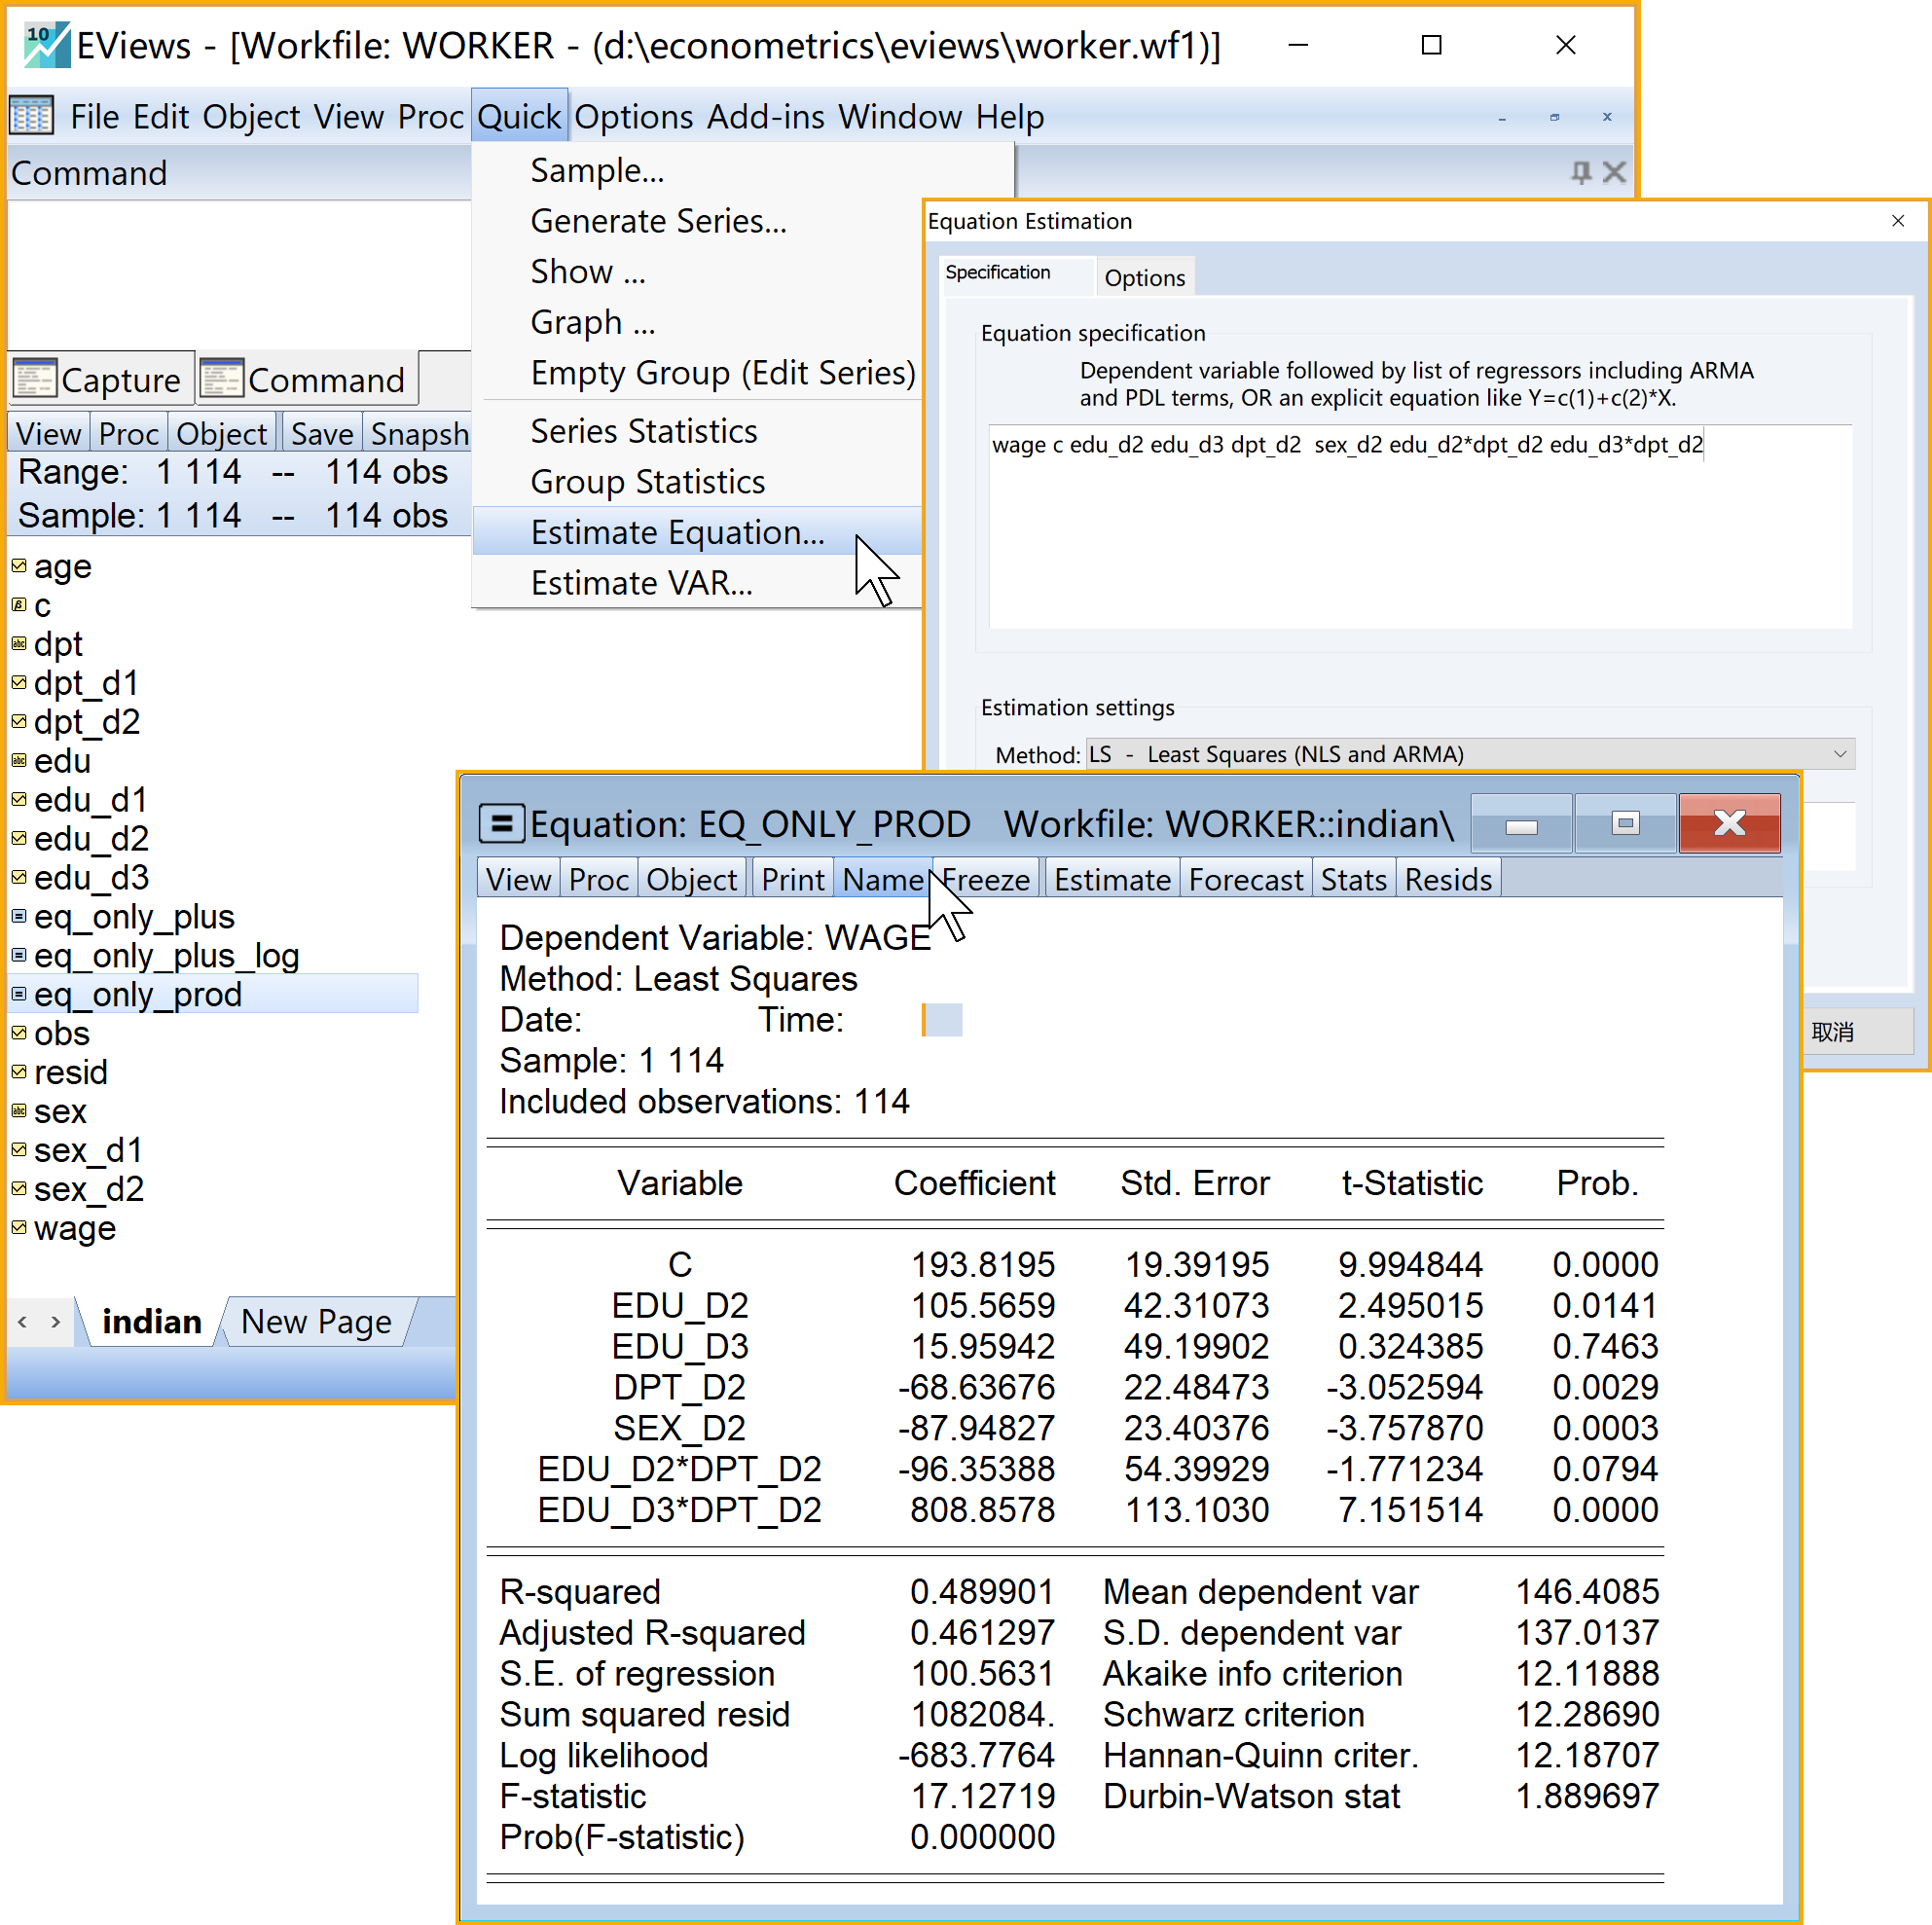
\includegraphics[width=27.57in]{picture/lab8-dummy-model/2-only-prod} 

}

\caption{只含虚拟变量的、乘法形式的经典线性回归模型Eviews实现}\label{fig:only-prod}
\end{figure}

\begin{figure}

{\centering 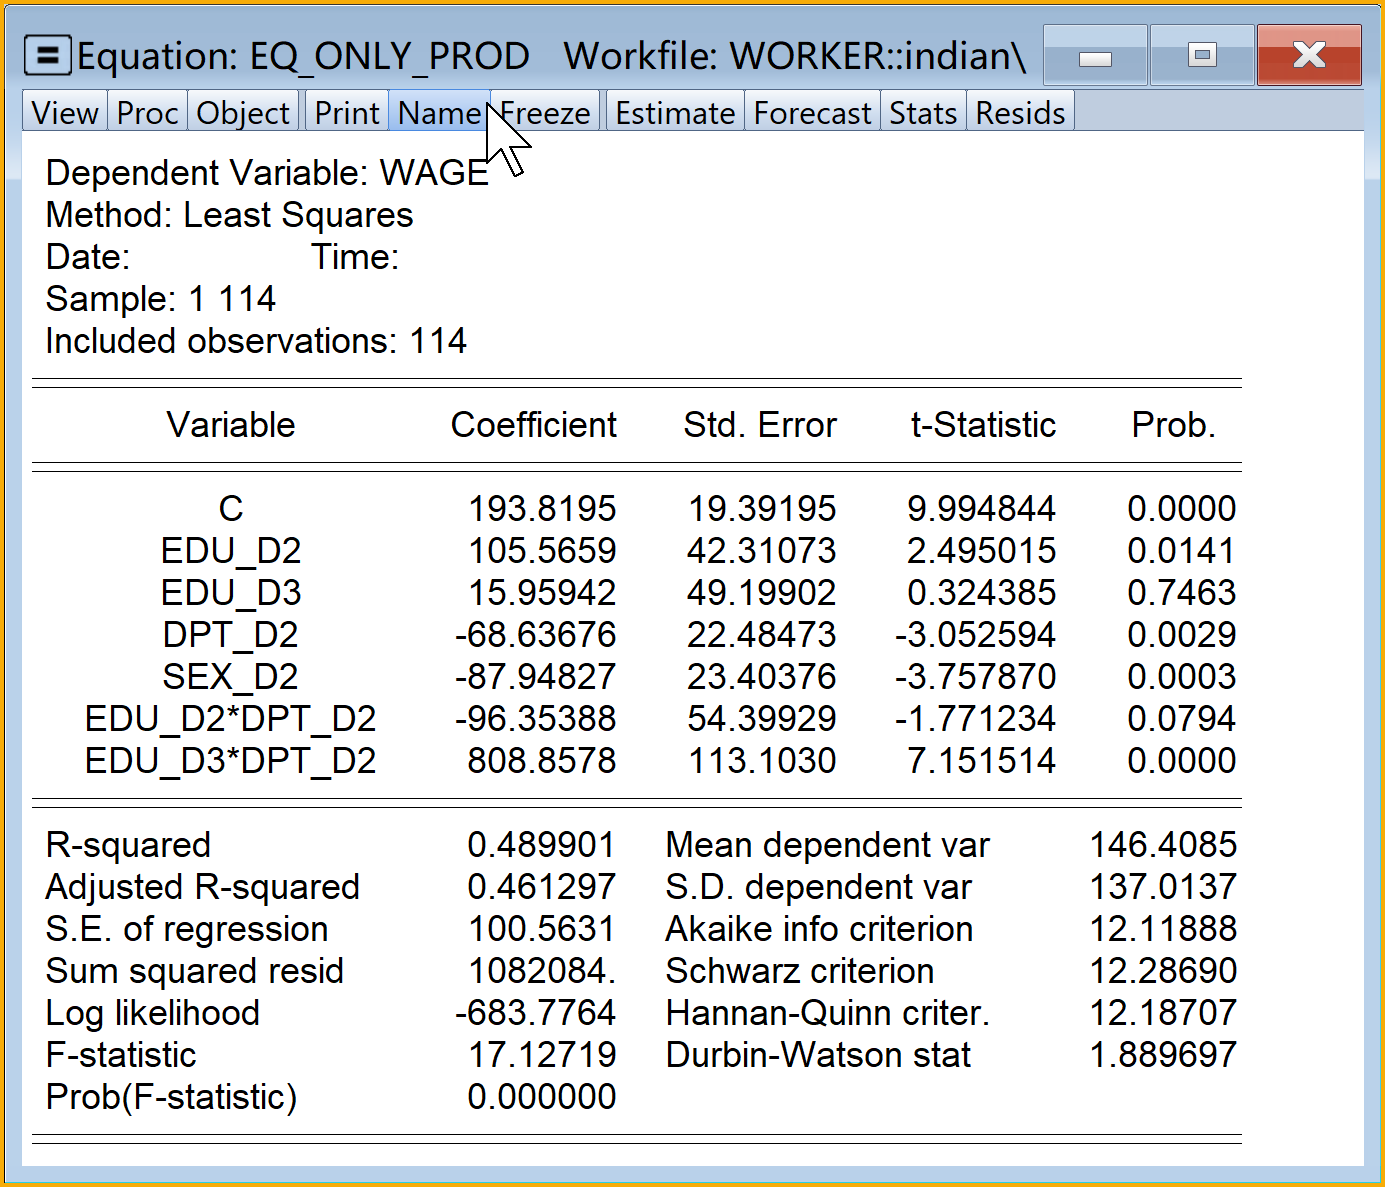
\includegraphics[width=19.24in]{picture/lab8-dummy-model/2-only-prod-report} 

}

\caption{只含虚拟变量的、乘法形式的经典线性回归模型Eviews报告}\label{fig:only-prod-report}
\end{figure}

\begin{itemize}
\tightlist
\item
  Eviews操作2(只含有虚拟变量的、乘法形式的\textbf{半对数回归模型}见方程\eqref{eq:only-prod-log-part},菜单操作实现具体见图\ref{fig:only-prod-log-part}):

  \begin{enumerate}
  \def\labelenumi{\arabic{enumi})}
  \tightlist
  \item
    确定参照组为{[}\textbf{文盲\&短期合同\&女性}{]},则如下虚拟变量将\textbf{不进入}回归模型

    \begin{enumerate}
    \def\labelenumii{\alph{enumii}.}
    \tightlist
    \item
      
\includegraphics{picture/object/Series.png}\texttt{edu\_d1}
    \item
      
\includegraphics{picture/object/Series.png}\texttt{dpt\_d1}
    \item
      
\includegraphics{picture/object/Series.png}\texttt{sex\_d1}
    \end{enumerate}
  \item
    设置回归模型。进入引导设置Equation Estimation \(\Rightarrow\)
    specification

    \begin{enumerate}
    \def\labelenumii{\alph{enumii}.}
    \tightlist
    \item
      Equation
      specification:输入命令\texttt{log(wage)\ c\ dpt\_d2\ \ sex\_d2\ edu\_d2*dpt\_d2\ edu\_d3*dpt\_d2\ edu\_d4*dpt\_d2}
    \item
      Estimation settings:

      \begin{itemize}
      \tightlist
      \item
        Method: 下拉选择LS - Least Squares (NLS and ARMA)
      \item
        Sample: (默认设置)
      \end{itemize}
    \item
      点击完成:OK
    \item
      命名保存方程对象
\includegraphics{picture/object/Equation.png}:(建议命名为\texttt{eq\_only\_prod\_log\_part})
    \item
      查看结果:双击
\includegraphics{picture/object/Equation.png}\texttt{eq\_only\_prod\_log\_part}
    \end{enumerate}
  \end{enumerate}
\end{itemize}

具体Eviews报告见\ref{fig:only-prod-log-part-report}:

\begin{figure}

{\centering 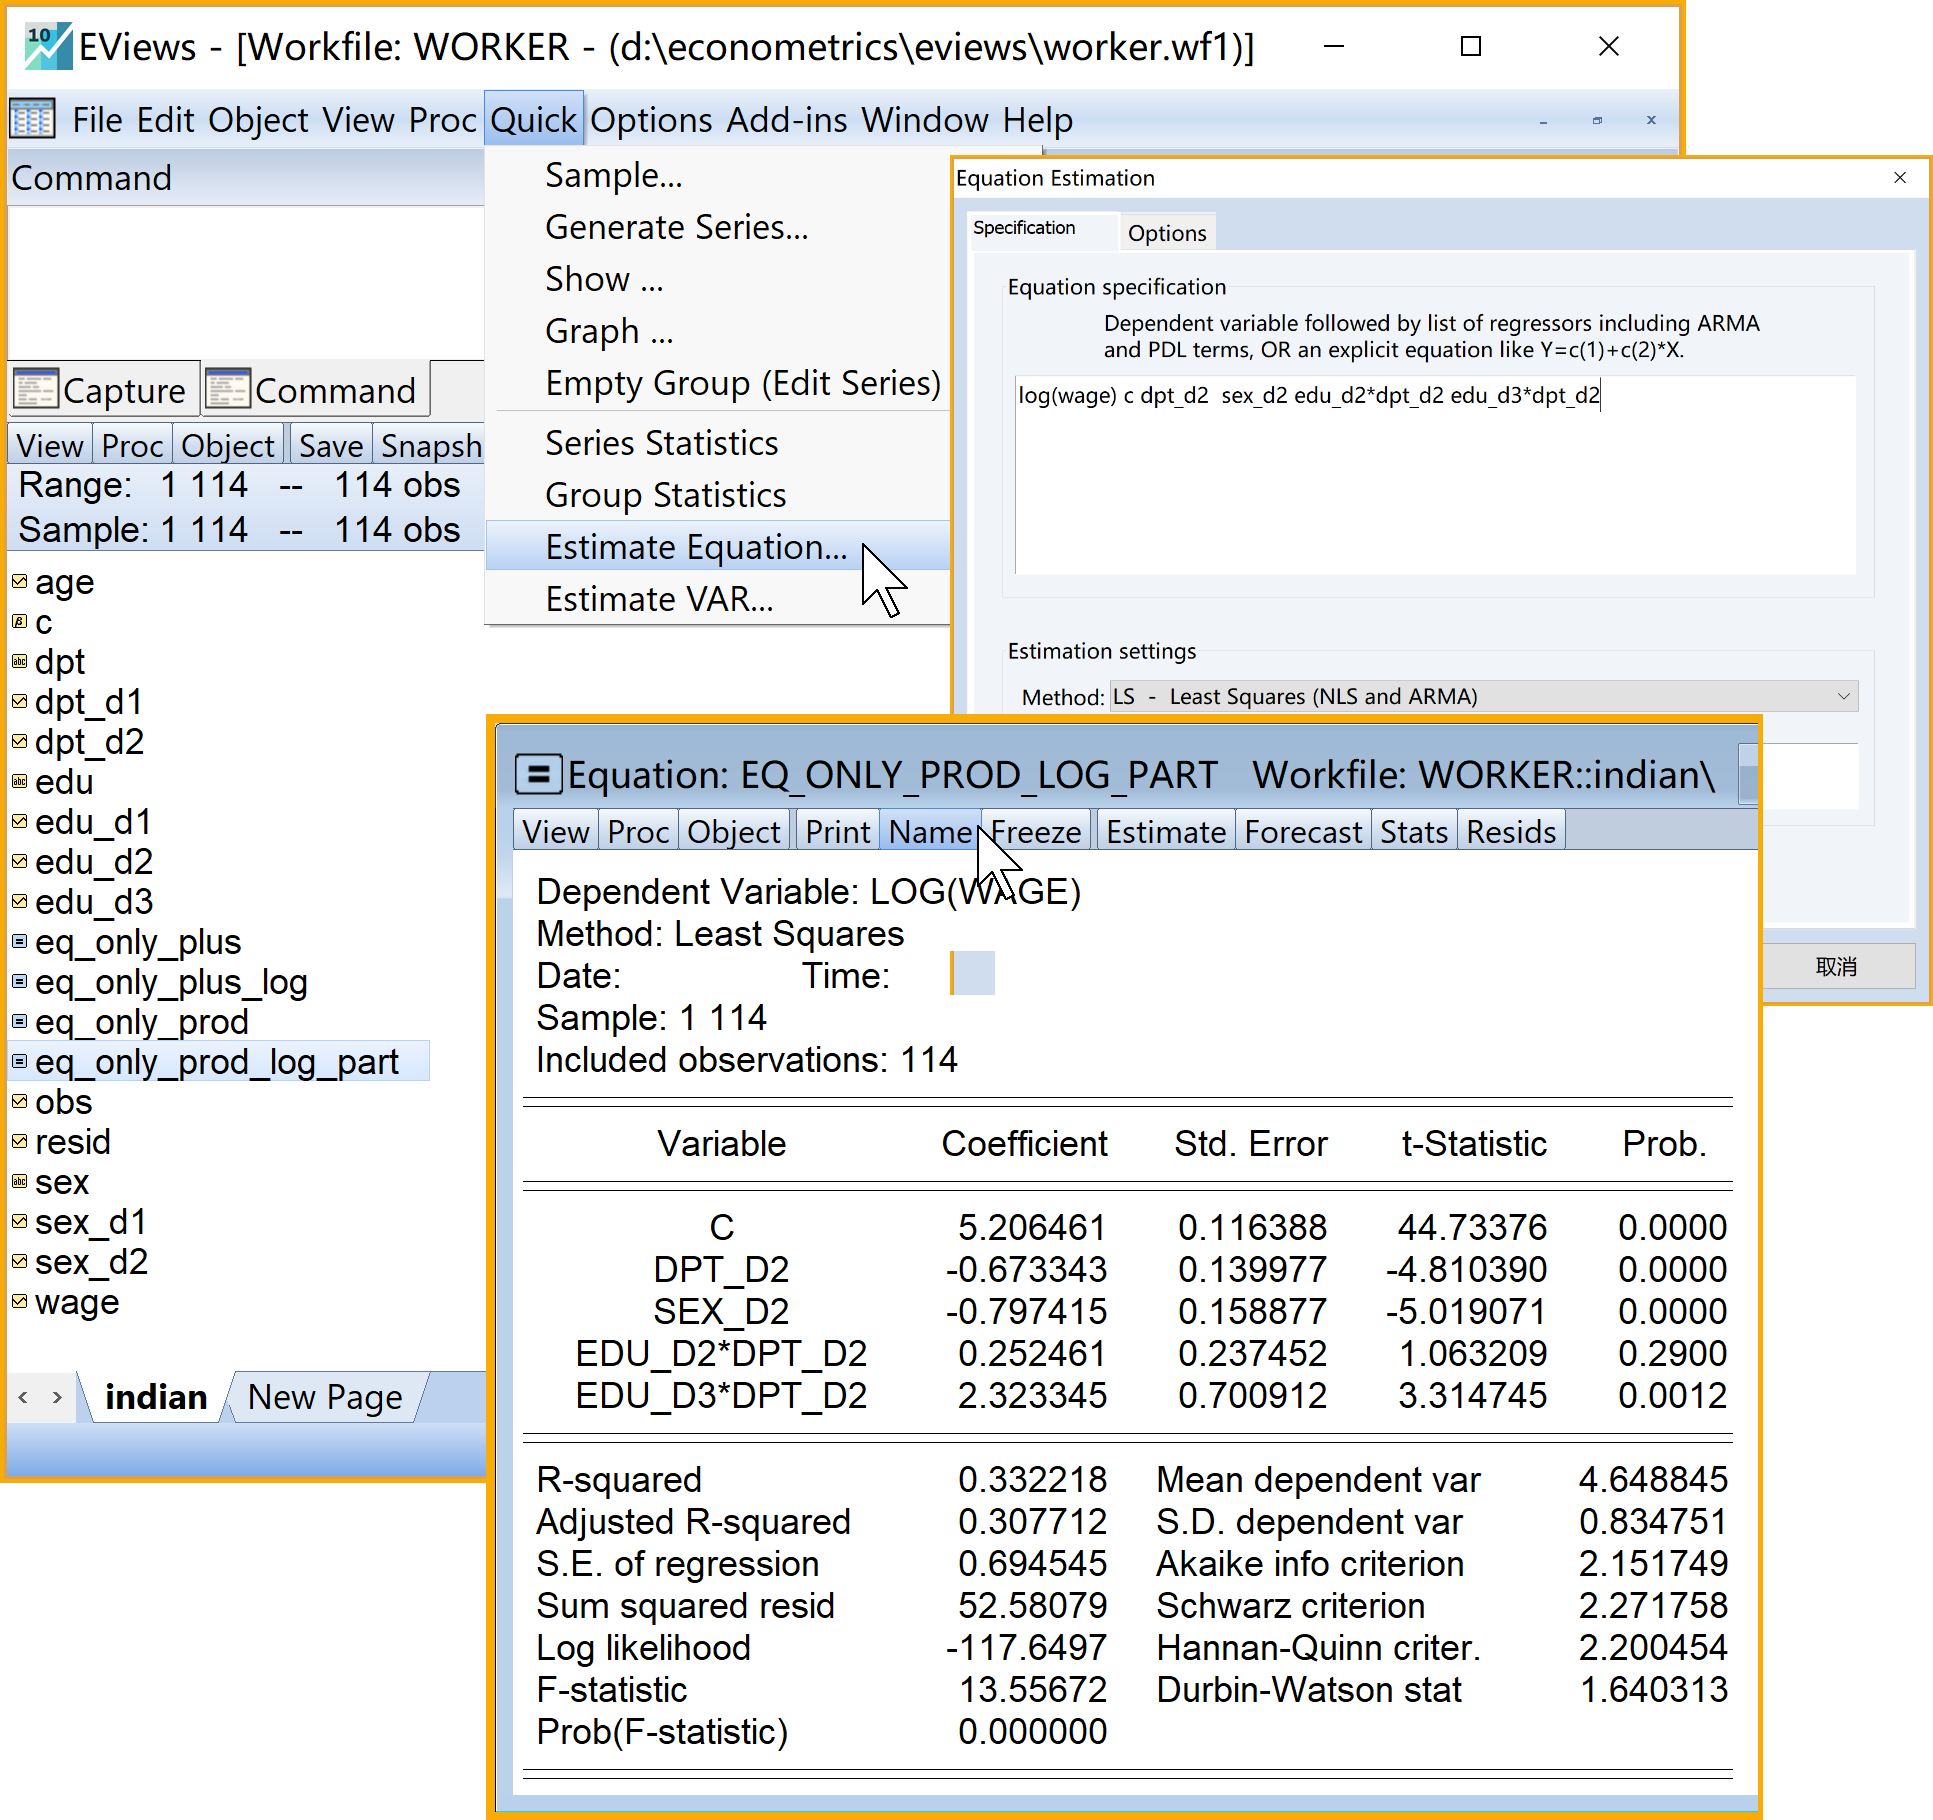
\includegraphics[width=26.85in]{picture/lab8-dummy-model/2-only-prod-log-part} 

}

\caption{只含虚拟变量的、乘法形式的半对数线性回归模型Eviews实现}\label{fig:only-prod-log-part}
\end{figure}

\begin{figure}

{\centering 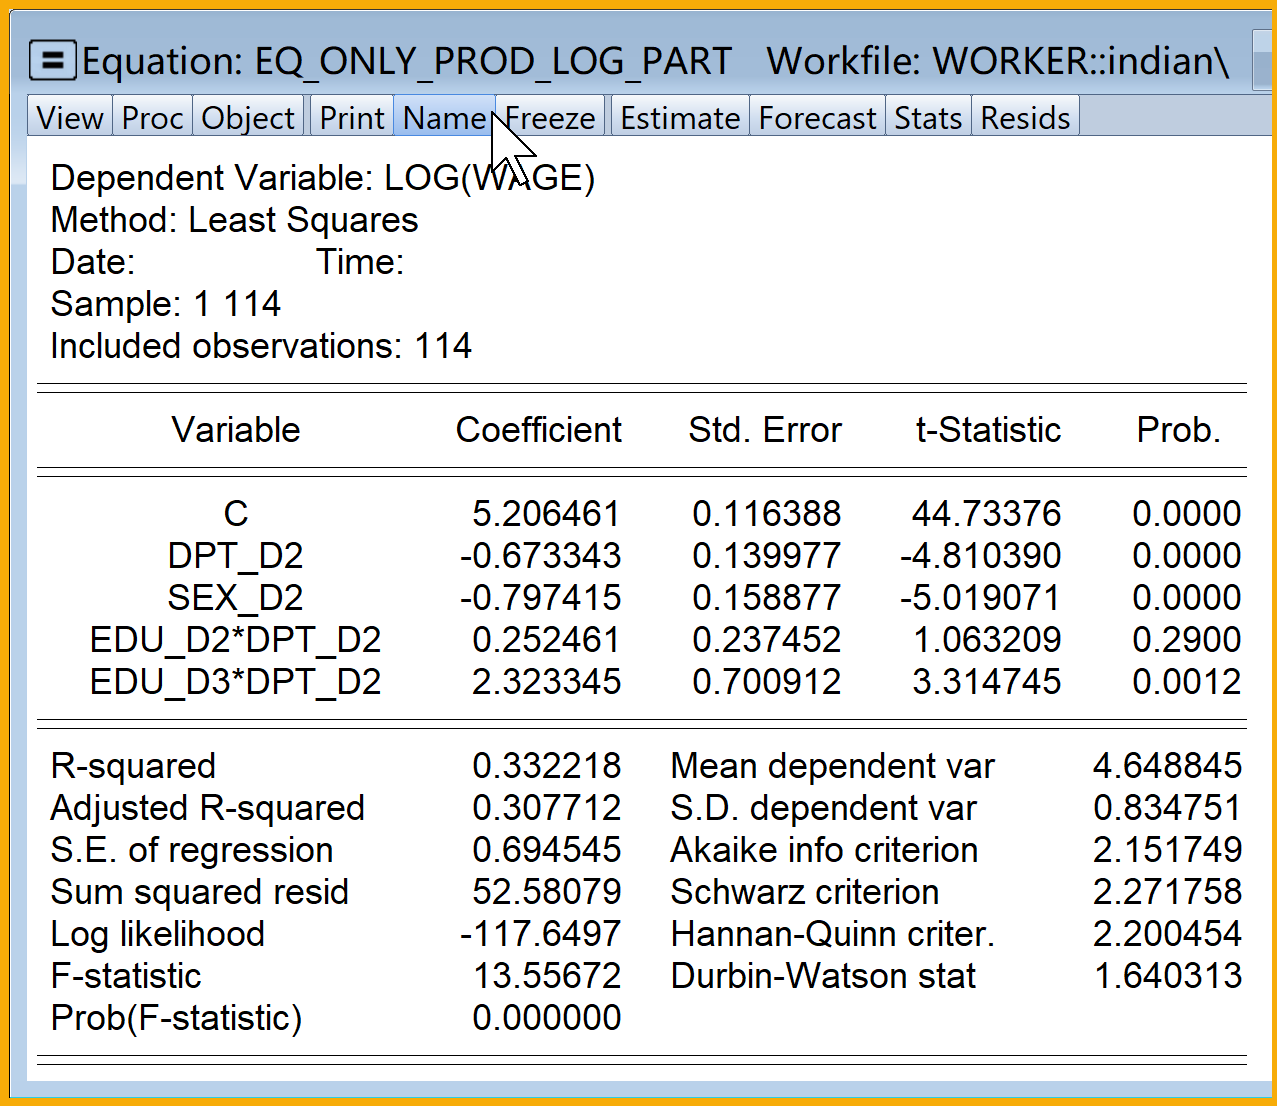
\includegraphics[width=17.74in]{picture/lab8-dummy-model/2-only-prod-log-part-report} 

}

\caption{只含虚拟变量的、乘法形式的半对数线性回归模型Eviews报告}\label{fig:only-prod-log-part-report}
\end{figure}

\hypertarget{-1}{%
\subparagraph{报告解读}\label{-1}}

只含虚拟变量的、乘法形式的经典回归模型(全部变量进入)Eviews结果简要报告如下:

\textbackslash{}begin\{alignedat\}\{5\} \&
\widehat{wage}=+\&120.70+\&23.03edu\_D2+\&13.72edu\_D3+\&829.30edu\_D4+\&74.78dpt\_D2
\textbackslash{} \&
\text{(t)}\&(7.9082)\&(0.7060)\&(0.3895)\&(8.0985)\&(2.9864)
\textbackslash{} \&
\text{(se)}\&(15.2625)\&(32.6264)\&(35.2241)\&(102.4020)\&(25.0404)
\textbackslash{} \&
\quad-\&88.19sex\_D2-\&32.62edu\_D2:dpt\_D2+\&90.22edu\_D3:dpt\_D2-\&814.86edu\_D4:dpt\_D2
\textbackslash{} \&
\text{(t)}\&(-3.6975)\&(-0.5459)\&(1.6171)\&(-7.1313) \textbackslash{}
\& \text{(se)}\&(23.8515)\&(59.7485)\&(55.7896)\&(114.2653)
\textbackslash{} \& \text{(fitness)}\& \quad\& R\^{}2=0.4925\&
\bar\{R\^{}2\}=0.4538\& F\^{}\{\ast\}=12.7366
\textbackslash{}end\{alignedat\}

只含虚拟变量的、乘法形式的经典回归模型(部分变量进入)Eviews结果简要报告如下:

\textbackslash{}begin\{alignedat\}\{5\} \&
\widehat{wage}=+\&120.70+\&74.78dpt\_D2-\&88.19sex\_D2+\&23.03edu\_D2+\&13.72edu\_D3
\textbackslash{} \&
\text{(t)}\&(7.9082)\&(2.9864)\&(-3.6975)\&(0.7060)\&(0.3895)
\textbackslash{} \&
\text{(se)}\&(15.2625)\&(25.0404)\&(23.8515)\&(32.6264)\&(35.2241)
\textbackslash{} \&
\quad+\&829.30edu\_D4-\&32.62dpt\_D2:edu\_D2+\&90.22dpt\_D2:edu\_D3-\&814.86dpt\_D2:edu\_D4
\textbackslash{} \& \text{(t)}\&(8.0985)\&(-0.5459)\&(1.6171)\&(-7.1313)
\textbackslash{} \&
\text{(se)}\&(102.4020)\&(59.7485)\&(55.7896)\&(114.2653)
\textbackslash{} \& \text{(fitness)}\& \quad\& R\^{}2=0.4925\&
\bar\{R\^{}2\}=0.4538\& F\^{}\{\ast\}=12.7366
\textbackslash{}end\{alignedat\}

只含虚拟变量的、乘法形式的半对数回归模型(部分变量进入)Eviews结果简要报告如下:
\textbackslash{}begin\{alignedat\}\{5\} \&
\widehat{log(wage)}=+\&4.52+\&0.52dpt\_D2-\&0.79sex\_D2+\&0.06edu\_D2+\&0.27edu\_D3
\textbackslash{} \&
\text{(t)}\&(43.4667)\&(3.0729)\&(-4.8492)\&(0.2838)\&(1.1078)
\textbackslash{} \&
\text{(se)}\&(0.1040)\&(0.1706)\&(0.1625)\&(0.2222)\&(0.2399)
\textbackslash{} \&
\quad+\&2.34edu\_D4+\&0.00dpt\_D2:edu\_D2+\&0.38dpt\_D2:edu\_D3-\&1.96dpt\_D2:edu\_D4
\textbackslash{} \& \text{(t)}\&(3.3514)\&(0.0097)\&(1.0126)\&(-2.5246)
\textbackslash{} \& \text{(se)}\&(0.6975)\&(0.4070)\&(0.3800)\&(0.7783)
\textbackslash{} \& \text{(fitness)}\& \quad\& R\^{}2=0.3656\&
\bar\{R\^{}2\}=0.3173\& F\^{}\{\ast\}=7.5648
\textbackslash{}end\{alignedat\}

\hypertarget{group2}{%
\subsubsection{同时含有虚拟变量和定量变量的回归模型(考虑基础组的情形)}\label{group2}}

\hypertarget{-1}{%
\paragraph{加法模型}\label{-1}}

\begin{itemize}
\tightlist
\item
  理论提示:

  \begin{itemize}
  \tightlist
  \item
    模型1:同时含有虚拟变量和定量变量的、加法形式的\textbf{经典回归模型}见方程\eqref{eq:both-plus}
  \item
    模型2:同时含有虚拟变量和定量变量的、加法形式的\textbf{半对数回归模型}见方程\eqref{eq:both-plus-log}
  \end{itemize}
\end{itemize}

\begin{align}
wage_i & =\alpha_1+\alpha_2edu_{D2,i}+\alpha_3edu_{D3,i}+\alpha_4edu_{D4,i}+\beta_2 dpt_{D2,i}+\gamma_2 sex_{D2,i}+\delta age_i+u_i   \label{eq:both-plus} \\
ln(wage_i) & =\alpha_1+\alpha_2edu_{D2,i}+\alpha_3edu_{D3,i}+\alpha_4edu_{D4,i}+\beta_2 dpt_{D2,i}+\gamma_2 sex_{D2,i}+\delta age_i+u_i  \label{eq:both-plus-log}
\end{align}

\begin{itemize}
\tightlist
\item
  Eviews操作1(同时含有虚拟变量和定量变量的、加法形式的\textbf{经典回归模型}见方程\eqref{eq:both-plus},菜单操作实现具体见图\ref{fig:both-plus}):

  \begin{enumerate}
  \def\labelenumi{\arabic{enumi})}
  \tightlist
  \item
    确定参照组为{[}\textbf{文盲\&短期合同\&女性}{]},则如下虚拟变量将\textbf{不进入}回归模型

    \begin{enumerate}
    \def\labelenumii{\alph{enumii}.}
    \tightlist
    \item
      
\includegraphics{picture/object/Series.png}\texttt{edu\_d1}
    \item
      
\includegraphics{picture/object/Series.png}\texttt{dpt\_d1}
    \item
      
\includegraphics{picture/object/Series.png}\texttt{sex\_d1}
    \end{enumerate}
  \item
    设置回归模型。进入引导设置Equation Estimation \(\Rightarrow\)
    specification

    \begin{enumerate}
    \def\labelenumii{\alph{enumii}.}
    \tightlist
    \item
      Equation
      specification:输入命令\texttt{wage\ c\ edu\_d2\ edu\_d3\ edu\_d4\ dpt\_d2\ sex\_d2\ age}
    \item
      Estimation settings:

      \begin{itemize}
      \tightlist
      \item
        Method: 下拉选择LS - Least Squares (NLS and ARMA)
      \item
        Sample: (默认设置)
      \end{itemize}
    \item
      点击完成:OK
    \item
      命名保存方程对象\includegraphics{picture/object/Equation.png}:(建议命名为\texttt{eq\_both\_plus})
    \item
      查看结果:双击\includegraphics{picture/object/Equation.png}\texttt{eq\_both\_plus}
    \end{enumerate}
  \end{enumerate}
\end{itemize}

具体Eviews报告见\ref{fig:both-plus-report}:

\begin{figure}

{\centering \includegraphics[width=27.75in]{picture/lab8-dummy-model/3-both-plus} 

}

\caption{同时含虚拟变量和定量变量的、加法形式的经典线性回归模型Eviews实现}\label{fig:both-plus}
\end{figure}

\begin{figure}

{\centering \includegraphics[width=18.36in]{picture/lab8-dummy-model/3-both-plus-report} 

}

\caption{同时含虚拟变量和定量变量的、加法形式的经典线性回归模型Eviews报告}\label{fig:both-plus-report}
\end{figure}

\begin{itemize}
\tightlist
\item
  Eviews操作2(同时含有虚拟变量和定量变量的、加法形式的\textbf{半对数回归模型}见方程\eqref{eq:both-plus-log},菜单操作实现具体见图\ref{fig:both-plus-log}):

  \begin{enumerate}
  \def\labelenumi{\arabic{enumi})}
  \tightlist
  \item
    确定参照组为{[}\textbf{文盲\&短期合同\&女性}{]},则如下虚拟变量将\textbf{不进入}回归模型

    \begin{enumerate}
    \def\labelenumii{\alph{enumii}.}
    \tightlist
    \item
      \includegraphics{picture/object/Series.png}\texttt{edu\_d1}
    \item
      \includegraphics{picture/object/Series.png}\texttt{dpt\_d1}
    \item
      \includegraphics{picture/object/Series.png}\texttt{sex\_d1}
    \end{enumerate}
  \item
    设置回归模型。进入引导设置Equation Estimation \(\Rightarrow\)
    specification

    \begin{enumerate}
    \def\labelenumii{\alph{enumii}.}
    \tightlist
    \item
      Equation
      specification:输入命令\texttt{log(wage)\ c\ edu\_d2\ edu\_d3\ edu\_d4\ dpt\_d2\ sex\_d2\ age}
    \item
      Estimation settings:

      \begin{itemize}
      \tightlist
      \item
        Method: 下拉选择LS - Least Squares (NLS and ARMA)
      \item
        Sample: (默认设置)
      \end{itemize}
    \item
      点击完成:OK
    \item
      命名保存方程对象\includegraphics{picture/object/Equation.png}:(建议命名为\texttt{eq\_both\_plus\_log})
    \item
      查看结果:双击\includegraphics{picture/object/Equation.png}\texttt{eq\_both\_plus\_log}
    \end{enumerate}
  \end{enumerate}
\end{itemize}

具体Eviews报告见\ref{fig:both-plus-log-report}:

\begin{figure}

{\centering \includegraphics[width=27.26in]{picture/lab8-dummy-model/3-both-plus-log} 

}

\caption{同时含虚拟变量和定量变量的、加法形式的半对数线性回归模型Eviews实现}\label{fig:both-plus-log}
\end{figure}

\begin{figure}

{\centering \includegraphics[width=18.53in]{picture/lab8-dummy-model/3-both-plus-log-report} 

}

\caption{同时含虚拟变量和定量变量的、加法形式的半对数线性回归模型Eviews报告}\label{fig:both-plus-log-report}
\end{figure}

\hypertarget{-2}{%
\subparagraph{报告解读}\label{-2}}

同时含虚拟变量和定量变量的、加法形式的经典回归模型Eviews结果简要报告如下:

\textbackslash{}begin\{alignedat\}\{5\} \&
\widehat{wage}=+\&6.79+\&23.96edu\_D2+\&61.59edu\_D3+\&150.49edu\_D4+\&31.16dpt\_D2
\textbackslash{} \&
\text{(t)}\&(0.2130)\&(0.7734)\&(1.9867)\&(3.0054)\&(1.3141)
\textbackslash{} \&
\text{(se)}\&(31.8931)\&(30.9789)\&(31.0035)\&(50.0725)\&(23.7120)
\textbackslash{} \& \quad-\&83.20sex\_D2+\&3.99age \textbackslash{} \&
\text{(t)}\&(-3.0819)\&(4.5129) \textbackslash{} \&
\text{(se)}\&(26.9981)\&(0.8835) \textbackslash{} \& \text{(fitness)}\&
\quad\& R\^{}2=0.3450\& \bar\{R\^{}2\}=0.3083\& F\^{}\{\ast\}=9.3945
\textbackslash{}end\{alignedat\}

同时含虚拟变量和定量变量的、加法形式的半对数回归模型Eviews结果简要报告如下:

\textbackslash{}begin\{alignedat\}\{5\} \&
\widehat{log(wage)}=+\&3.62+\&0.16edu\_D2+\&0.51edu\_D3+\&0.62edu\_D4+\&0.32dpt\_D2
\textbackslash{} \&
\text{(t)}\&(21.3135)\&(0.9530)\&(3.0586)\&(2.3342)\&(2.5264)
\textbackslash{} \&
\text{(se)}\&(0.1699)\&(0.1651)\&(0.1652)\&(0.2668)\&(0.1263)
\textbackslash{} \& \quad-\&0.67sex\_D2+\&0.03age \textbackslash{} \&
\text{(t)}\&(-4.6302)\&(6.2268) \textbackslash{} \&
\text{(se)}\&(0.1438)\&(0.0047) \textbackslash{} \& \text{(fitness)}\&
\quad\& R\^{}2=0.4991\& \bar\{R\^{}2\}=0.4710\& F\^{}\{\ast\}=17.7694
\textbackslash{}end\{alignedat\}

\hypertarget{-1}{%
\paragraph{乘法模型}\label{-1}}

\begin{itemize}
\tightlist
\item
  理论提示:

  \begin{itemize}
  \tightlist
  \item
    模型1:同时含有虚拟变量和定量变量的、乘法形式的\textbf{经典回归模型}见方程\eqref{eq:both-prod}
  \item
    模型2:同时含有虚拟变量和定量变量的、乘法形式的\textbf{半对数回归模型}见方程\eqref{eq:both-prod-log-part}
  \end{itemize}
\end{itemize}

\[\begin{equation}
\begin{split}
wage_i & =\alpha_1+\alpha_2edu_{D2,i}+\alpha_3edu_{D3,i}+\alpha_4edu_{D4,i}+\beta_2 dpt_{D2,i}+\gamma_2sex_{D2,i}+\delta age_i
\\ & +\lambda_2edu_{D2,i} \ast dpt_{D2,i}+\lambda_3edu_{D3,i}\ast dpt_{D2,i}+\lambda_4edu_{D4,i}\ast dpt_{D2,i}  +u_i  
\end{split}
\label{eq:both-prod} 
\end{equation}\]

\begin{align}
\begin{split}
wage_i & =\alpha_1+\beta_2 dpt_{D2,i}+\gamma_2sex_{D2,i} +\delta age_i \\
& +\lambda_2edu_{D2,i} \ast dpt_{D2,i}+\lambda_3edu_{D3,i}\ast dpt_{D2,i}+\lambda_4edu_{D4,i}\ast dpt_{D2,i} +u_i 
\end{split}
\label{eq:both-prod-part} 
\end{align}

\begin{align}
\begin{split}
ln(wage_i) & =\alpha_1+\beta_2 dpt_{D2,i}+\gamma_2sex_{D2,i} +\delta age_i \\
& +\lambda_2edu_{D2,i} \ast dpt_{D2,i}+\lambda_3edu_{D3,i}\ast dpt_{D2,i} +\lambda_4edu_{D4,i}\ast dpt_{D2,i}+u_i 
\end{split}
\label{eq:both-prod-log-part} 
\end{align}

\begin{itemize}
\tightlist
\item
  Eviews操作1(同时含有虚拟变量和定量变量的、乘法形式的\textbf{经典回归模型}见方程\eqref{eq:both-prod},菜单操作实现具体见图\ref{fig:both-prod}):

  \begin{enumerate}
  \def\labelenumi{\arabic{enumi})}
  \tightlist
  \item
    确定参照组为{[}\textbf{文盲\&短期合同\&女性}{]},则如下虚拟变量将\textbf{不进入}回归模型

    \begin{enumerate}
    \def\labelenumii{\alph{enumii}.}
    \tightlist
    \item
      \includegraphics{picture/object/Series.png}\texttt{edu\_d1}
    \item
      \includegraphics{picture/object/Series.png}\texttt{dpt\_d1}
    \item
      \includegraphics{picture/object/Series.png}\texttt{sex\_d1}
    \end{enumerate}
  \item
    设置回归模型。进入引导设置Equation Estimation \(\Rightarrow\)
    specification

    \begin{enumerate}
    \def\labelenumii{\alph{enumii}.}
    \tightlist
    \item
      Equation
      specification:输入命令\texttt{wage\ c\ edu\_d2\ edu\_d3\ edu\_d4\ dpt\_d2\ sex\_d2\ age\ edu\_d2*dpt\_d2\ edu\_d3*dpt\_d2\ edu\_d4*dpt\_d2}
    \item
      Estimation settings:

      \begin{itemize}
      \tightlist
      \item
        Method: 下拉选择LS - Least Squares (NLS and ARMA)
      \item
        Sample: (默认设置)
      \end{itemize}
    \item
      点击完成:OK
    \item
      命名保存方程对象\includegraphics{picture/object/Equation.png}:(建议命名为\texttt{eq\_both\_prod})
    \item
      查看结果:双击\includegraphics{picture/object/Equation.png}\texttt{eq\_both\_prod}
    \end{enumerate}
  \end{enumerate}
\end{itemize}

具体Eviews报告见\ref{fig:both-prod-report}:

\begin{figure}

{\centering \includegraphics[width=27.15in]{picture/lab8-dummy-model/3-both-prod} 

}

\caption{同时含虚拟变量和定量变量的、乘法形式的经典线性回归模型Eviews实现}\label{fig:both-prod}
\end{figure}

\begin{figure}

{\centering \includegraphics[width=18.53in]{picture/lab8-dummy-model/3-both-prod-report} 

}

\caption{同时含虚拟变量和定量变量的、乘法形式的经典线性回归模型Eviews报告}\label{fig:both-prod-report}
\end{figure}

\begin{itemize}
\tightlist
\item
  Eviews操作2(同时含有虚拟变量和定量变量的、乘法形式的\textbf{半对数回归模型}见方程\eqref{eq:both-prod-log-part},菜单操作实现具体见图\ref{fig:both-prod-log-part}):

  \begin{enumerate}
  \def\labelenumi{\arabic{enumi})}
  \tightlist
  \item
    确定参照组为{[}\textbf{文盲\&短期合同\&女性}{]},则如下虚拟变量将\textbf{不进入}回归模型

    \begin{enumerate}
    \def\labelenumii{\alph{enumii}.}
    \tightlist
    \item
      \includegraphics{picture/object/Series.png}\texttt{edu\_d1}
    \item
      \includegraphics{picture/object/Series.png}\texttt{dpt\_d1}
    \item
      \includegraphics{picture/object/Series.png}\texttt{sex\_d1}
    \end{enumerate}
  \item
    设置回归模型。进入引导设置Equation Estimation \(\Rightarrow\)
    specification

    \begin{enumerate}
    \def\labelenumii{\alph{enumii}.}
    \tightlist
    \item
      Equation
      specification:输入命令\texttt{log(wage)\ c\ dpt\_d2\ sex\_d2\ age\ edu\_d2*dpt\_d2\ edu\_d3*dpt\_d2\ edu\_d4*dpt\_d2}
    \item
      Estimation settings:

      \begin{itemize}
      \tightlist
      \item
        Method: 下拉选择LS - Least Squares (NLS and ARMA)
      \item
        Sample: (默认设置)
      \end{itemize}
    \item
      点击完成:OK
    \item
      命名保存方程对象\includegraphics{picture/object/Equation.png}:(建议命名为\texttt{eq\_both\_prod\_log\_part})
    \item
      查看结果:双击\includegraphics{picture/object/Equation.png}\texttt{eq\_both\_prod\_log\_part}
    \end{enumerate}
  \end{enumerate}
\end{itemize}

具体Eviews报告见\ref{fig:both-prod-log-part-report}:

\begin{figure}

{\centering \includegraphics[width=26.89in]{picture/lab8-dummy-model/3-both-prod-log-part} 

}

\caption{同时含虚拟变量和定量变量的、乘法形式的半对数线性回归模型Eviews实现}\label{fig:both-prod-log-part}
\end{figure}

\begin{figure}

{\centering \includegraphics[width=18.53in]{picture/lab8-dummy-model/3-both-prod-log-part-report} 

}

\caption{同时含虚拟变量和定量变量的、乘法形式的半对数线性回归模型Eviews报告}\label{fig:both-prod-log-part-report}
\end{figure}

\hypertarget{-3}{%
\subparagraph{报告解读}\label{-3}}

同时含虚拟变量和定量变量的、乘法形式的经典回归模型(全部变量进入)Eviews结果简要报告如下:

\textbackslash{}begin\{alignedat\}\{5\} \&
\widehat{wage}=+\&19.43+\&32.29edu\_D2+\&35.59edu\_D3+\&777.93edu\_D4+\&54.46dpt\_D2
\textbackslash{} \&
\text{(t)}\&(0.7215)\&(1.0706)\&(1.0830)\&(8.1760)\&(2.3131)
\textbackslash{} \&
\text{(se)}\&(26.9248)\&(30.1607)\&(32.8591)\&(95.1488)\&(23.5466)
\textbackslash{} \&
\quad-\&70.34sex\_D2+\&3.25age-\&26.81edu\_D2:dpt\_D2+\&59.80edu\_D3:dpt\_D2-\&766.28edu\_D4:dpt\_D2
\textbackslash{} \&
\text{(t)}\&(-3.1451)\&(4.4121)\&(-0.4864)\&(1.1521)\&(-7.2326)
\textbackslash{} \&
\text{(se)}\&(22.3647)\&(0.7361)\&(55.1151)\&(51.9083)\&(105.9477)
\textbackslash{} \& \text{(fitness)}\& \quad\& R\^{}2=0.5725\&
\bar\{R\^{}2\}=0.5355\& F\^{}\{\ast\}=15.4756
\textbackslash{}end\{alignedat\}

同时含虚拟变量和定量变量的、乘法形式的经典回归模型(部分变量进入)Eviews结果简要报告如下:

\textbackslash{}begin\{alignedat\}\{5\} \&
\widehat{wage}=+\&19.43+\&54.46dpt\_D2-\&70.34sex\_D2+\&3.25age+\&32.29edu\_D2
\textbackslash{} \&
\text{(t)}\&(0.7215)\&(2.3131)\&(-3.1451)\&(4.4121)\&(1.0706)
\textbackslash{} \&
\text{(se)}\&(26.9248)\&(23.5466)\&(22.3647)\&(0.7361)\&(30.1607)
\textbackslash{} \&
\quad+\&35.59edu\_D3+\&777.93edu\_D4-\&26.81dpt\_D2:edu\_D2+\&59.80dpt\_D2:edu\_D3-\&766.28dpt\_D2:edu\_D4
\textbackslash{} \&
\text{(t)}\&(1.0830)\&(8.1760)\&(-0.4864)\&(1.1521)\&(-7.2326)
\textbackslash{} \&
\text{(se)}\&(32.8591)\&(95.1488)\&(55.1151)\&(51.9083)\&(105.9477)
\textbackslash{} \& \text{(fitness)}\& \quad\& R\^{}2=0.5725\&
\bar\{R\^{}2\}=0.5355\& F\^{}\{\ast\}=15.4756
\textbackslash{}end\{alignedat\}

同时含虚拟变量和定量变量的、乘法形式的半对数回归模型(部分变量进入)Eviews结果简要报告如下:
\textbackslash{}begin\{alignedat\}\{5\} \&
\widehat{log(wage)}=+\&3.65+\&0.35dpt\_D2-\&0.63sex\_D2+\&0.03age+\&0.14edu\_D2
\textbackslash{} \&
\text{(t)}\&(21.0939)\&(2.3114)\&(-4.4157)\&(5.8925)\&(0.7352)
\textbackslash{} \&
\text{(se)}\&(0.1730)\&(0.1513)\&(0.1437)\&(0.0047)\&(0.1938)
\textbackslash{} \&
\quad+\&0.45edu\_D3+\&1.90edu\_D4+\&0.05dpt\_D2:edu\_D2+\&0.12dpt\_D2:edu\_D3-\&1.55dpt\_D2:edu\_D4
\textbackslash{} \&
\text{(t)}\&(2.1475)\&(3.1022)\&(0.1519)\&(0.3711)\&(-2.2738)
\textbackslash{} \&
\text{(se)}\&(0.2112)\&(0.6114)\&(0.3542)\&(0.3336)\&(0.6808)
\textbackslash{} \& \text{(fitness)}\& \quad\& R\^{}2=0.5244\&
\bar\{R\^{}2\}=0.4833\& F\^{}\{\ast\}=12.7417
\textbackslash{}end\{alignedat\}

\hypertarget{seasonal}{%
\subsubsection{时间序列季节虚拟变量模型}\label{seasonal}}

\begin{itemize}
\tightlist
\item
  目的:通过学习时间序列季节虚拟变量模型,进一步深入理解虚拟变量回归模型的多种形式及应用\\
\item
  思路:设置并引入季节虚拟变量,构建时间序列季节虚拟变量模型,Eviews估计回归结果\\
\item
  定义:

  \begin{itemize}
  \tightlist
  \item
    季节模式(seasonal
    pattern):大多数时间序列经济变量,通常表现出来的季节性往复行为或现象。
  \item
    季节调整(seasonal
    adjusted):将时间序列经济变量的季节性变化成分去除,从而得到一个新的变量序列的处理过程。
  \end{itemize}
\item
  理论提示:

  \begin{itemize}
  \tightlist
  \item
    事实上,一个时间序列经济变量往往同时存在四个成分,分别是季节成分(seasonal
    component)、周期成分(cyclical component)、趋势成分(trend
    component)和严格随机成分(strictly random component)。
  \item
    根据基础组的有无,可以构建以第一季度为基础组的时间序列季节虚拟变量模型\eqref{eq:S1}和无基础组的时间序列季节虚拟变量模型\eqref{eq:S0}。其中,\(X_t\)为定量变量。
  \end{itemize}
\end{itemize}

\begin{align}
Y_t=\beta_1+\beta_2X_t+\lambda_2D2_t+\lambda_3D3_t+\lambda_4D4_t+u_t \label{eq:S1}\\
Y_t=\beta_2X_t+\lambda_1D1_t+\lambda_2D2_t+\lambda_3D3_t+\lambda_4D4_t+u_t \label{eq:S0}
\end{align}

\begin{itemize}
\tightlist
\item
  Eviews操作(略)
\end{itemize}

\hypertarget{piecewise}{%
\subsubsection{分段线性回归模型(piecewise linear
regression)}\label{piecewise}}

\begin{itemize}
\tightlist
\item
  目的:通过学习分段式线性回归模型,进一步深入理解虚拟变量回归模型的多种形式及应用
\item
  思路:设置并引入虚拟变量,构建分段线性回归模型,Eviews估计回归结果
\item
  定义:

  \begin{itemize}
  \tightlist
  \item
    \textbf{分段}现象:在经济关系中,当解释变量\(X\)的值达到某一水平/阀值\(X^\ast\)之前,与被解释变量之间存在某种线性关系;当解释变量X的值达到或者超过水平/阀值\(X^\ast\)以后,与被解释变量的关系就会发生变化。因而总体看来,似乎被明显``分段''了。
  \item
    分段线性回归模型(piecewise linear
    regression):是指用虚拟变量估计不同水平/阀值的解释变量\(X\)对被解释变量\(Y\)的影响的一类线性回归模型。
  \end{itemize}
\item
  理论提示:

  \begin{itemize}
  \tightlist
  \item
    一个阀值的分段线性回归模型\eqref{eq:PIR1}
  \item
    两个阀值的分段线性回归模型\eqref{eq:PIR2}
  \end{itemize}
\end{itemize}

\begin{align}
Y_i & =\beta_1+\beta_2X_i+\lambda(X_i-X^{\ast})D_i+u_i \label{eq:PIR1}\\
Y_i & =\beta_1+\beta_2X_i+\lambda_1(X_i-X^{\ast}_1)D1_i+\lambda_2(X_i-X^{\ast}_2)D2_i+u_i \label{eq:PIR2}
\end{align}

\begin{itemize}
\tightlist
\item
  Eviews操作(略)
\end{itemize}

\subsection{作业题}

\textbf{印度工人工资}:表\ref{tab:data-worker-lab}给出给出了114位印度工人在wage工人工资,age年龄,edu教育水平,dpt合同类型,sex性别等方面的数据。

\begin{table}

\caption{\label{tab:data-worker-lab}印度工人工资(n=114)}
\centering
\begin{tabular}[t]{rrrlll}
\toprule
obs & wage & age & edu & dpt & sex\\
\midrule
1 & 117.00 & 26 & primary & permanent & female\\
2 & 375.00 & 42 & primary & permanent & female\\
3 & 175.00 & 33 & primary & permanent & female\\
4 & 100.00 & 33 & primary & permanent & female\\
5 & 162.50 & 30 & primary & permanent & female\\
\addlinespace
110 & 25.00 & 18 & illiteracy & temporary & male\\
111 & 25.00 & 11 & illiteracy & temporary & male\\
112 & 75.00 & 45 & illiteracy & temporary & male\\
113 & 53.84 & 14 & illiteracy & temporary & male\\
114 & 50.00 & 26 & illiteracy & temporary & male\\
\bottomrule
\end{tabular}
\end{table}

变量说明见表\ref{tab:label-worker-lab}:

\begin{table}

\caption{\label{tab:label-worker-lab}变量定义及说明}
\centering
\begin{tabular}[t]{l|l|l}
\hline
variable & label & remark\\
\hline
obs & 工人编号 & 序号\\
\hline
wage & 工人工资 & 美元/周\\
\hline
age & 年龄 & 岁\\
\hline
edu & 教育水平 & illiteracy=文盲;primary=初等教育;secondary=中等教育;higher=高等教育\\
\hline
dpt & 合同类型 & temporary=短期合同;permanent=长期合同\\
\hline
sex & 性别 & female=女;male=男\\
\hline
\end{tabular}
\end{table}

请回答如下问题:

\begin{enumerate}
\def\labelenumi{\arabic{enumi}.}
\item
  请对数据表\ref{tab:data-worker-lab}进行数据处理,将定性变量都处理成\textbf{完全}虚拟变量体系(也即定性变量有m个属性,则设置m个虚拟变量)。(要求:定性变量edu的虚拟变量设置为edu\_D1,edu\_D2,\(\cdots\);定性变量dpt的虚拟变量设置为dpt\_D1,\(\cdots\);定性变量sex的虚拟变量设置为sex\_D1,\(\cdots\)。虚拟变量的下标请与变量说明表\ref{tab:label-worker-lab}的保持一致)
\item
  使用\textbf{全部变量},并提出一个\textbf{加法形式}的有截距虚拟变量回归模型,用以预测工人工资。要求基础组设置为(\textbf{文盲\&短期合同\&女性})的工人组。

  \begin{enumerate}
  \def\labelenumii{\alph{enumii}.}
  \tightlist
  \item
    请写出加法形式的有截距虚拟变量回归模型(PRM)
  \item
    请利用你自己构建的模型,进行eviews分析,得到分析报告。(要求将报告截图过来,并写出相应的简要报告形式------三行式或四行式)
  \item
    根据回归分析结果,请预测如下几类工人的工资水平:(要求分别写出理论表达式,以及数据分析的预测值)

    \begin{itemize}
    \tightlist
    \item
      (\textbf{文盲\&短期合同\&女性\&50岁})的工人
    \item
      (\textbf{高等教育\&长期合同\&男性\&50岁})的工人
    \item
      (\textbf{初等教育\&短期合同\&男性\&30岁})的工人
    \item
      (\textbf{初等教育\&长期合同\&女性\&30岁})的工人
    \end{itemize}
  \end{enumerate}
\item
  使用\textbf{全部变量},并提出一个\textbf{乘法形式}的有截距虚拟变量回归模型,用以预测工人工资。要求基础组设置为(\textbf{文盲\&短期合同\&女性})的工人组,且要求教育程度edu的虚拟变量(edu\_D1,edu\_D2,\(\cdots\))与合同类型dpt的虚拟变量(dpt\_D1,\(\cdots\))进行乘法交互。

  \begin{enumerate}
  \def\labelenumii{\alph{enumii}.}
  \tightlist
  \item
    请写出该乘法形式的有截距虚拟变量回归模型(PRM)
  \item
    请利用你自己构建的模型,进行eviews分析,得到分析报告。(要求将报告截图过来,并写出相应的简要报告形式------三行式或四行式)
  \item
    根据回归分析结果,请预测如下几类工人的工资水平:(要求分别写出理论表达式,以及数据分析的预测值)

    \begin{itemize}
    \tightlist
    \item
      (\textbf{文盲\&短期合同\&女性\&50岁})的工人
    \item
      (\textbf{高等教育\&长期合同\&男性\&50岁})的工人
    \item
      (\textbf{初等教育\&短期合同\&男性\&30岁})的工人
    \item
      (\textbf{初等教育\&长期合同\&女性\&30岁})的工人
    \end{itemize}
  \end{enumerate}
\item
  使用\textbf{全部变量},对因变量ln(wage)提出一个\textbf{乘法形式}的有截距虚拟变量回归模型,用以预测工人工资。要求基础组设置为(\textbf{文盲\&短期合同\&女性})的工人组,且要求性别sex的虚拟变量(sex\_D1,\(\cdots\))与合同类型dpt的虚拟变量(dpt\_D1,\(\cdots\))进行乘法交互。

  \begin{enumerate}
  \def\labelenumii{\alph{enumii}.}
  \tightlist
  \item
    请写出该乘法形式的有截距虚拟变量回归模型(PRM)
  \item
    请利用你自己构建的模型,进行eviews分析,得到分析报告,并回答如下问题。(要求将报告截图过来,并写出相应的简要报告形式------三行式或四行式)

    \begin{itemize}
    \tightlist
    \item
      你认为这些新引入的交互项看上去有显著的交互影响吗?
    \item
      男性工人与女性工人相比,收入存在明显差异吗?请给出你的理由。
    \item
      长期合同的男性工人与长期合同的女性工人,收入存在明显差异吗?请给出你的理由。
    \item
      短期合同的男性工人与长期合同的女性工人,收入存在明显差异吗?请给出你的理由。
    \end{itemize}
  \item
    根据回归分析结果,请预测如下几类工人的工资水平:(要求分别写出理论表达式,以及数据分析的预测值)

    \begin{itemize}
    \tightlist
    \item
      (\textbf{文盲\&短期合同\&女性\&50岁})的工人
    \item
      (\textbf{高等教育\&长期合同\&男性\&50岁})的工人
    \item
      (\textbf{初等教育\&短期合同\&男性\&30岁})的工人
    \item
      (\textbf{初等教育\&长期合同\&女性\&30岁})的工人
    \end{itemize}
  \end{enumerate}
\item
  使用\textbf{除教育edu变量之外}的其他全部变量,对因变量ln(wage)提出一个\textbf{乘法形式}的有截距虚拟变量回归模型,用以预测工人工资。要求基础组设置为(\textbf{文盲\&短期合同\&女性})的工人组,且要求教育程度edu的虚拟变量(edu\_D1,edu\_D2,\(\cdots\))与合同类型dpt的虚拟变量(dpt\_D1,\(\cdots\))进行乘法交互。

  \begin{enumerate}
  \def\labelenumii{\alph{enumii}.}
  \tightlist
  \item
    请写出该乘法形式的有截距虚拟变量回归模型(PRM)
  \item
    请利用你自己构建的模型,进行eviews分析,得到分析报告,并回答如下问题。(要求将报告截图过来,并写出相应的简要报告形式------三行式或四行式)

    \begin{itemize}
    \tightlist
    \item
      你认为这些新引入的交互项看上去有显著的交互影响吗?
    \item
      高等数育的工人与初等教育的工人,收入存在明显差异吗?请给出你的理由。
    \item
      {[}高等教育的长期合同工人{]}与{[}高等教育的短期合同工人{]},收入存在明显差异吗?请给出你的理由。
    \item
      {[}高等教育的短期合同工人{]}与{[}初等教育的长期合同工人{]},收入存在明显差异吗?请给出你的理由。
    \end{itemize}
  \item
    根据回归分析结果,请预测如下几类工人的工资水平:(要求分别写出理论表达式,以及数据分析的预测值)

    \begin{itemize}
    \tightlist
    \item
      (\textbf{文盲\&短期合同\&女性\&50岁})的工人
    \item
      (\textbf{高等教育\&长期合同\&男性\&50岁})的工人
    \item
      (\textbf{初等教育\&短期合同\&男性\&30岁})的工人
    \item
      (\textbf{初等教育\&长期合同\&女性\&30岁})的工人
    \end{itemize}
  \end{enumerate}
\end{enumerate}


\end{document}
